\documentclass[aspectratio=43]{beamer}
\usepackage[czech]{babel}
\usepackage[utf8]{inputenc}
\usepackage[T1]{fontenc}
\usepackage{graphicx}
\usepackage{xcolor}
\usepackage{tikz}
\usetikzlibrary{shapes,arrows,positioning,fit,backgrounds}



% Definice barev SPŠE
\definecolor{spseBurgundy}{RGB}{142, 85, 85}  % Upravená burgundy podle obrázku

% Odstranění navigačních symbolů
\setbeamertemplate{navigation symbols}{}

% Nastavení vzhledu
\useinnertheme{default}
\useoutertheme{default}

% Úprava pozadí a barev
\setbeamercolor{background canvas}{bg=white}
\setbeamercolor{frametitle}{fg=white,bg=spseBurgundy}
\setbeamercolor{title}{fg=black,bg=white}
\setbeamercolor{itemize item}{fg=spseBurgundy}
\setbeamercolor{itemize subitem}{fg=spseBurgundy}

% Nastavení rámečku titulu
\setbeamertemplate{frametitle}{
  \vspace*{-0.1cm}
  \begin{beamercolorbox}[wd=\paperwidth,ht=1cm,dp=0.2cm]{frametitle}
    \vspace*{0.1cm}\hspace*{1cm}\insertframetitle
  \end{beamercolorbox}
}

% Patička
\setbeamertemplate{footline}{%
   \begin{beamercolorbox}[wd=\paperwidth,ht=1cm,dp=0.2cm,left]{structure}
    \hspace*{0.5cm}
\includegraphics[height=0.6cm]{logo.png}%
    \hfill\hfill{\color{black}\insertshortsubtitle}\hfill%
    \hfill\hfill{\color{black}\insertframenumber/\inserttotalframenumber}\hspace*{0.5cm}%
  \end{beamercolorbox}
}

% Nastavení odrážek
\setbeamertemplate{itemize item}{\small\raise0.5pt\hbox{\donotcoloroutermaths$\blacksquare$}}
\setbeamertemplate{itemize subitem}{\small\raise0.5pt\hbox{\donotcoloroutermaths$\blacksquare$}}

\title{ROZHRANÍ A PERIFERIE PC}
\subtitle{ROZHRANÍ A PERIFERIE PC}
\author{Bc. David Zimniok}
\date{}

\begin{document}

% Titulní strana - speciální uspořádání
\begin{frame}[plain]
    \vspace*{-0.5cm}
    \begin{beamercolorbox}[wd=\paperwidth,ht=2cm]{frametitle}
        \hspace*{0.5cm}
\includegraphics[height=1.8cm]{logo_w.png}
    \end{beamercolorbox}
    \vspace{1cm}
    \begin{flushright}
        {\textbf{\Large \inserttitle} \par}
        \vspace{0.1cm}
        {\large HARDWARE 4. ročníky \par}
        {\large verze 01/25 \par}
        \vspace{1.5cm}
        {\scriptsize \insertauthor \par}
        {\scriptsize david.zimniok@spsehavirov.cz}
    \end{flushright}
    \vspace*{0.5cm}
    
\includegraphics[height=1cm]{logo.png}
\end{frame}


\section{Základní pojmy}
\begin{frame}{Základní pojmy - souvislosti}
	\begin{itemize}
		\item SCSI - vysokorychlostní paralelní rozhraní
		\item IDE - Zjednodušením SCSI pro 2 zařízení (potom EIDE)
		\item ATA - paralelní typ připojení (40pinový konektor, 40/80 žilový kabel)
		\item PATA - Paralel ATA (označení po příchodu SATA)
		\item SATA - sériové připojení (rychlejší, tenčí kabely)
		\item USB - Universal Serial Bus
		\item SAS - Serial Attached SCSI
		\item FireWire - IEEE1394
	\end{itemize}
\end{frame}


\section{PATA}
\begin{frame}{PATA - Parallel ATA}
	\begin{itemize}
		\item ATA - AT Attachment, standard IDE od Western Digital
		\item ATAPI - rozšíření pro jiná zařízení (CD, DVD)
		\item 16bitové rozhraní (původně pro ISA)
		\item 40žilový plochý kabel (tzv. "kšanda")
	\end{itemize}
\end{frame}


\begin{frame}{IDE aneb Paralelní ATA}
	\begin{itemize}
		\item IDE - Integrated Drive Electronics
		\item Master & Slave konfigurace
		\item EIDE - Enhanced IDE
		\item Primární a sekundární kanál
		\item Pokud je to možné, instalujte každou jednotku zvlášť -komunikace na jednom kanálu probíhá "na střídačku"
	\end{itemize}
	\begin{center}
		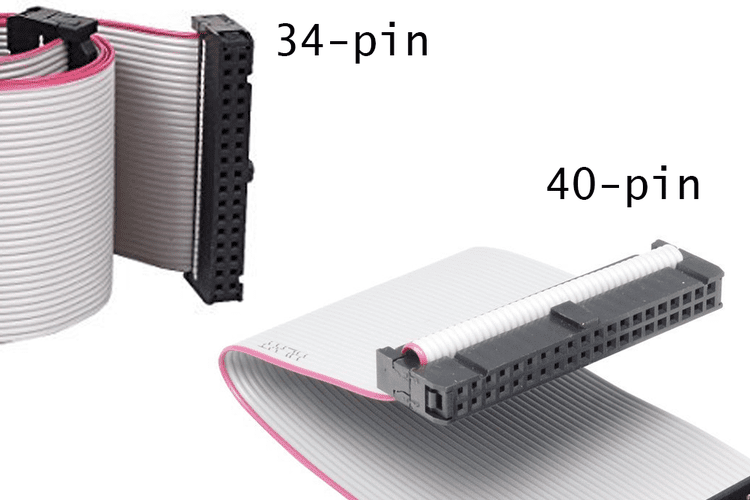
\includegraphics[width=0.6\linewidth]{extrahovane_obrazky/ide.png}
	\end{center}
\end{frame}


\begin{frame}{40 vs 80 žil}
	\begin{columns}
		\column{0.49\textwidth}
		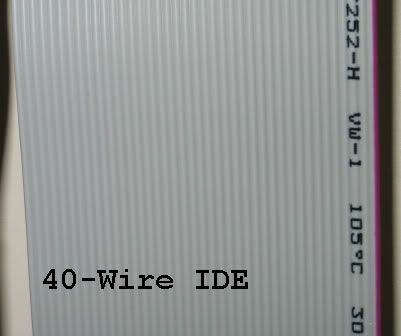
\includegraphics[width=1\linewidth]{extrahovane_obrazky/40IDE.jpeg}
		\column{0.49\textwidth}
		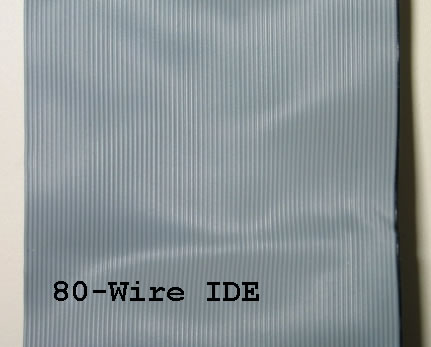
\includegraphics[width=1\linewidth]{extrahovane_obrazky/80IDE.jpeg}
	\end{columns}
	
\end{frame}


\begin{frame}{MS – SL – CS ?}
	\begin{itemize}
		\item CS – Cable Select, automatická detekce master/slave
		\item Pin 24 rozhoduje o roli zařízení
		\item Černý konektor – master
		\item Šedý konektor – slave
		\item Modrý konektor – základní deska
	\end{itemize}
	\begin{center}
		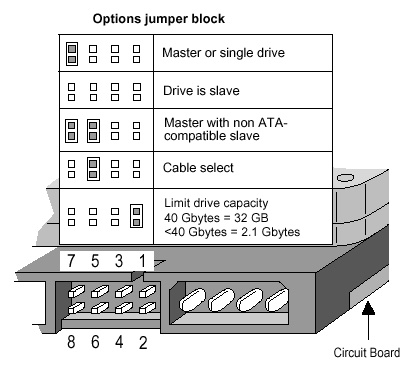
\includegraphics[width=0.55\linewidth]{extrahovane_obrazky/ide_j.jpg}
	\end{center}
\end{frame}


\begin{frame}{Způsoby připojení - EIDE}
	jumpery – propojení kontaktů, které umožňuje nastavit chování disku vůči druhému disku připojeného ke stejnému IDE kabelu
	\vfill
	\begin{columns}
		\column{0.49\textwidth}
		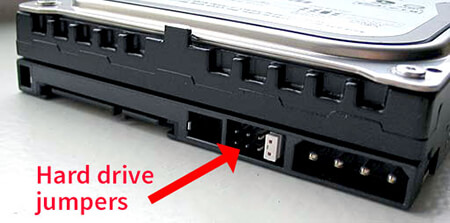
\includegraphics[width=1\linewidth]{extrahovane_obrazky/hdd_j.jpeg}
		\column{0.49\textwidth}
		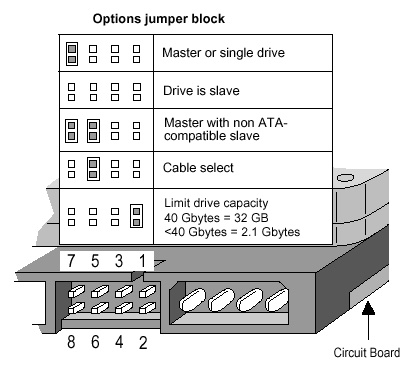
\includegraphics[width=1\linewidth]{extrahovane_obrazky/ide_j.jpg}
	\end{columns}
	
\end{frame}


\begin{frame}{IDE - PIO}
	\begin{itemize}
		\item PIO - Programmed Input and Output
		\item Tento způsob přenosu dat zatěžoval procesor
	\end{itemize}
	\vfill
	\begin{itemize}
		\item PIO 0 - přenosová rychlost 3,3 MB/s 
		\item PIO 1 - přenosová rychlost 5,2 MB/s 
		\item PIO 2 - přenosová rychlost 8,3 MB/s 
		\item PIO 3 - přenosová rychlost 11,1 MB/s
		\item PIO 4 - přenosová rychlost 16,6 MB/s 
		\item PIO 5 - přenosová rychlost 22,2 MB/s
	\end{itemize}
\end{frame}


\begin{frame}{IDE - DMA}
	\begin{itemize}
		\item Single Word
		      \begin{itemize}
		      	\item DMA 0 - přenosová rychlost 2,1 MB/s 
		      	\item DMA 1 - přenosová rychlost 4,2 MB/s 
		      	\item DMA 2 - přenosová rychlost 8,4 MB/s  
		      \end{itemize}
		\item Multi Word
		      \begin{itemize}
		      	\item DMA 0 - přenosová rychlost 4,2 MB/s 
		      	\item DMA 1 - přenosová rychlost 13,3 MB/s 
		      	\item DMA 2 - přenosová rychlost 16,6 MB/s 
		      \end{itemize}
		\item Ultra DMA
		      \begin{itemize}
		      	\item UDMA 0 - přenosová rychlost 16,6 MB/s 
		      	\item UDMA 2 - přenosová rychlost 33,3 MB/s 
		      	\item UDMA 4 - přenosová rychlost 66,6 MB/s (80 žil)
		      	\item UDMA 5 - přenosová rychlost 100 MB/s (80 žil)
		      	\item UDMA 6 - přenosová rychlost 133 MB/s (80 žil)
		      \end{itemize}
	\end{itemize}
	
	K připojení IDE disku se používá 80žilový IDE kabel, kde 40 vodičů vede signál, dalších 40 má za úkol stínit signál ostatních.  
\end{frame}


\begin{frame}{ATA}
	\begin{itemize}
		\item ATA-1 : kapacita 512 MB, módy: PIO 0-2, SW DMA 0-2, MW DMA 0 
		\item ATA-2 (EIDE, Fast ATA, Fast IDE): 8 GB (24bit. LBA), PIO 0-4, MW DMA 0-2 
		\item ATA-3 (EIDE): 128 GB (28bit LBA), S.M.A.R.T 
		\item ATA-4 (ATAPI-4): UDMA 0-2, podpora ATAPI CD-ROM 
		\item ATA-5 (ATAPI-5): UDMA 0-4, 80žilový kabel 
		\item ATA-6 (ATAPI-6): 144 PB (144 000 000 GB - 48bit LBA) 
		\item ATA-7 (ATAPI-7, SATA 150): UDMA 0-6, SATA
	\end{itemize}
	
\end{frame}


\begin{frame}{Přenosová rychlost PATA - problém}
	Např. ATA 100 \\
	Datová šířka rozhraní 16b = 2B \\
	Frekvence 25 MHz (DDR) \\
	$25 \cdot 2 = 50 \text{ Mhz (ef)} \cdot 2\text{B} = 100 \text{MB/s}$ \\
	\vfillČíslo za označením UltraATA, Ultra DMA udává max. 
	teoretickou přenosovou rychlost (100 = 100 MB/s) 
	\\
	Problém paralelních přenosů = vysoké frekvence, 
	délky kabelů a spojů.
	
\end{frame}

\section{FDD}
\begin{frame}{FDD rozhraní – 34 pin kabel}
	Konektor na překříženými adresovými vodiči je pro mechaniku A (jinak nutno v Setupu nastavit Swap A B)
	\begin{columns}
		\column{0.49\textwidth}
		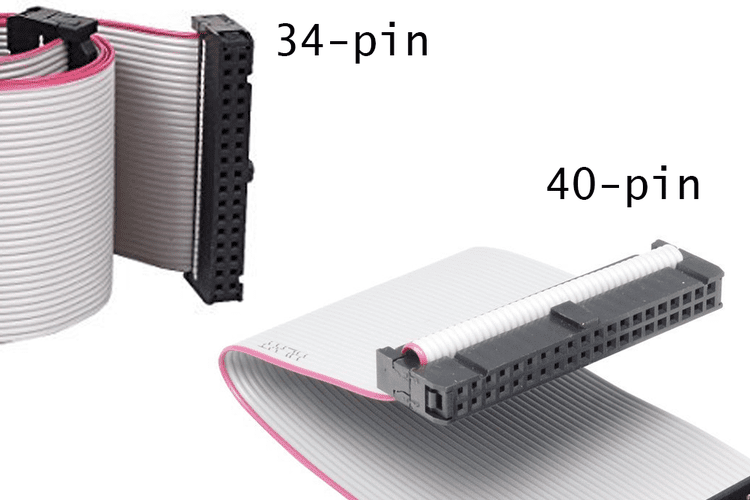
\includegraphics[width=1\linewidth]{extrahovane_obrazky/ide.png}
		\column{0.49\textwidth}
		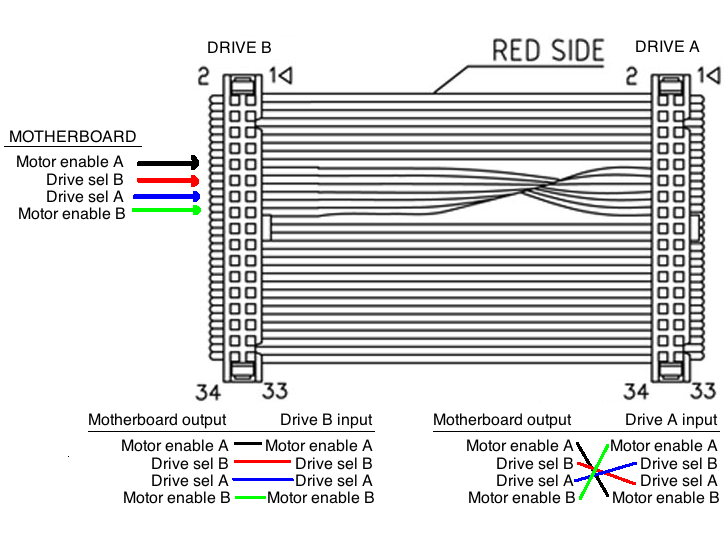
\includegraphics[width=1\linewidth]{extrahovane_obrazky/fdd_flip.png}
	\end{columns}
	
\end{frame}

\section{SCSI}
\begin{frame}{SCSI (Small Computer System Interface)}
	\begin{itemize}
		\item Vysokorychlostní paralerní rozhraní, používá se v serverech
		\item Existuje ve více revizích 
		\item Ultra320 SCSI nebo Ultra640 SCSI
		\item Číslo v názvu udává maximální rychlost v MB/s
	\end{itemize}
	\begin{columns}
		\column{0.49\textwidth}
		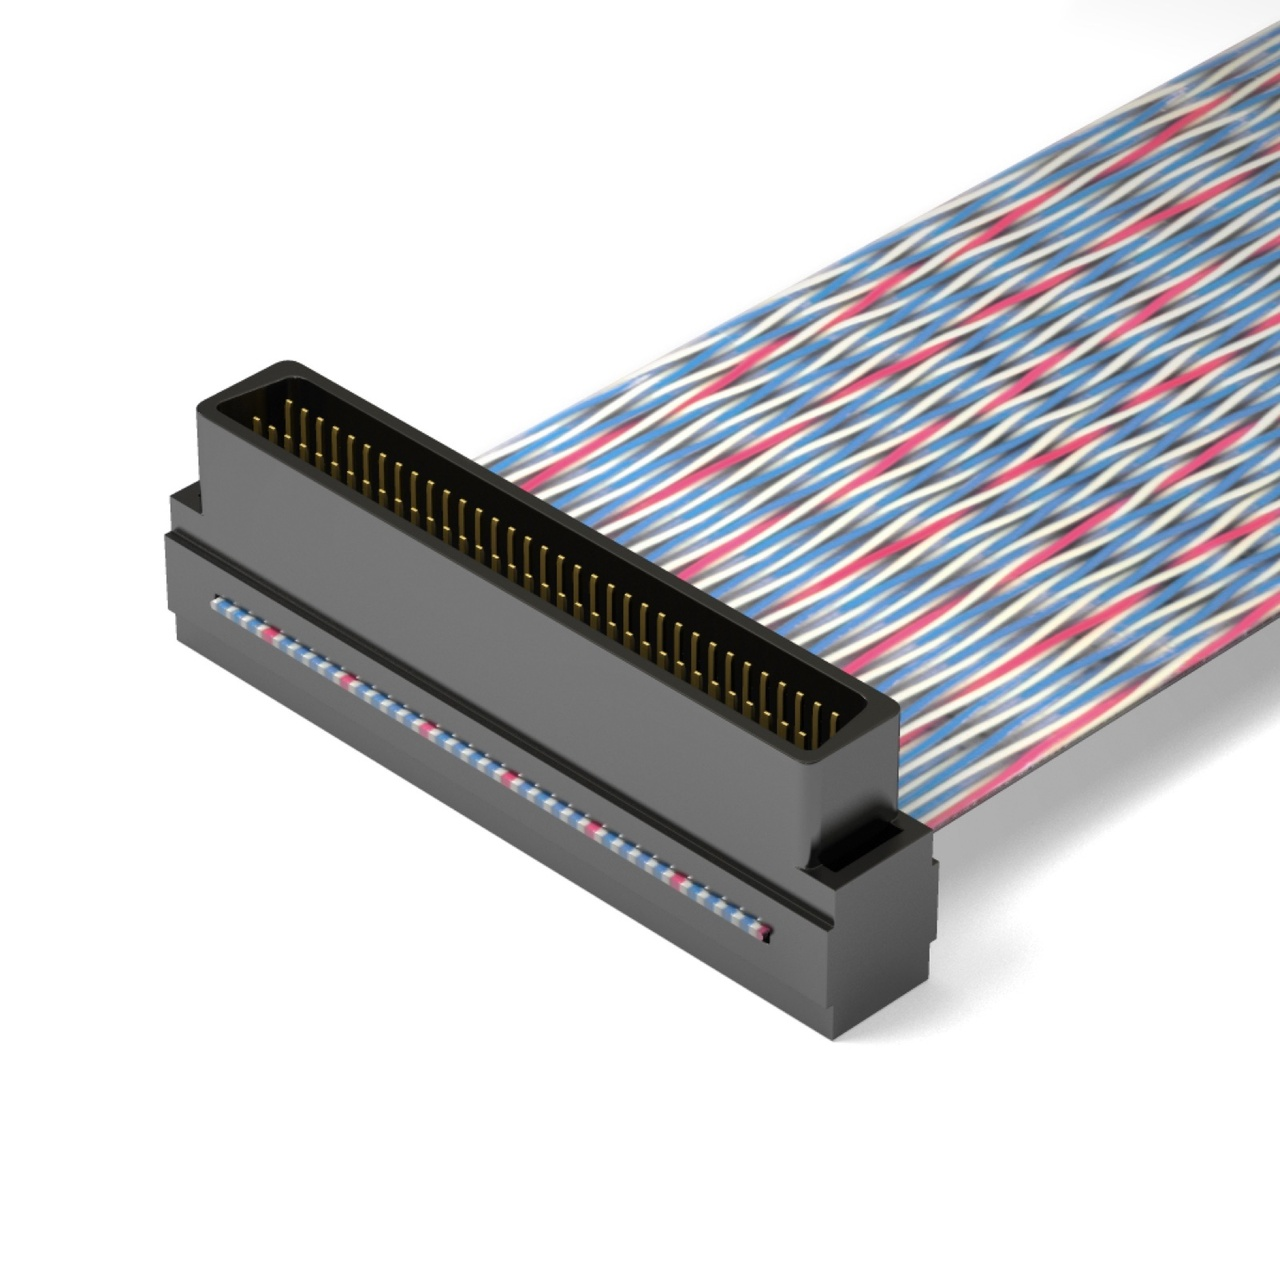
\includegraphics[width=1\linewidth]{extrahovane_obrazky/scsi_c.jpeg}
		\column{0.49\textwidth}
		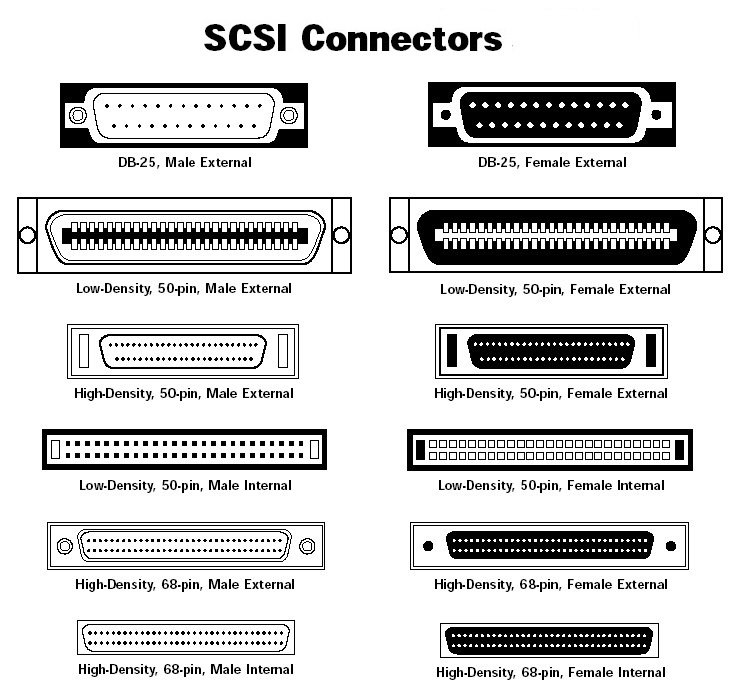
\includegraphics[width=1\linewidth]{extrahovane_obrazky/scsi_all.jpeg}
	\end{columns}
\end{frame}


\begin{frame}{Přehled standardů SCSI}
	\begin{table}[]
\begin{tabular}{|l|l|l|}
\hline
\textbf{Typ}                                                                & \textbf{Rychlost} & \textbf{Použití}        \\ \hline
\begin{tabular}[c]{@{}l@{}}Ultra320 SCSI \\ (16-bit Wide)\end{tabular}      & 320 MByte/sec     & Nejvýkonnější harddisky \\ \hline
\begin{tabular}[c]{@{}l@{}}Ultra160 SCSI \\ (16-bit Wide)\end{tabular}      & 160 MByte/sec     & Harddisky               \\ \hline
\begin{tabular}[c]{@{}l@{}}Ultra2 SCSI \\ (16-bit Wide)\end{tabular}        & 80 MByte/sec      & Harddisky               \\ \hline
\begin{tabular}[c]{@{}l@{}}Ultra Wide SCSI \\ (16-bit Wide)\end{tabular} &
  40 MByte/sec &
  \begin{tabular}[c]{@{}l@{}}Harddisky, \\ zálohovací mechaniky\end{tabular} \\ \hline
\begin{tabular}[c]{@{}l@{}}Ultra SCSI \\ (8-bit Narrow)\end{tabular} &
  20 MByte/sec &
  \begin{tabular}[c]{@{}l@{}}CD-R, CD-RW, \\ zálohovací mechaniky, \\ DVD mechaniky\end{tabular} \\ \hline
\begin{tabular}[c]{@{}l@{}}SCSI-2, Fast SCSI \\ (8-bit Narrow)\end{tabular} & 10 MByte/sec      & Skenery, CD-ROM         \\ \hline
\end{tabular}
\end{table}
\end{frame}


\begin{frame}{SCSI}
	
	
	\begin{columns}
		\column{0.49\textwidth}
		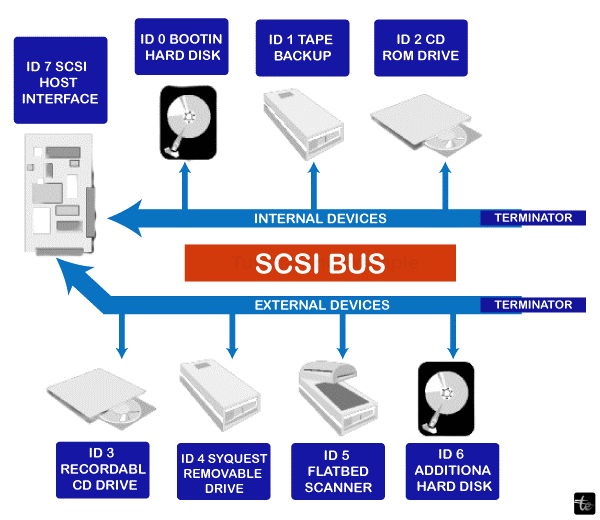
\includegraphics[width=1\linewidth]{extrahovane_obrazky/scsi_pr.png}
		\column{0.49\textwidth}
		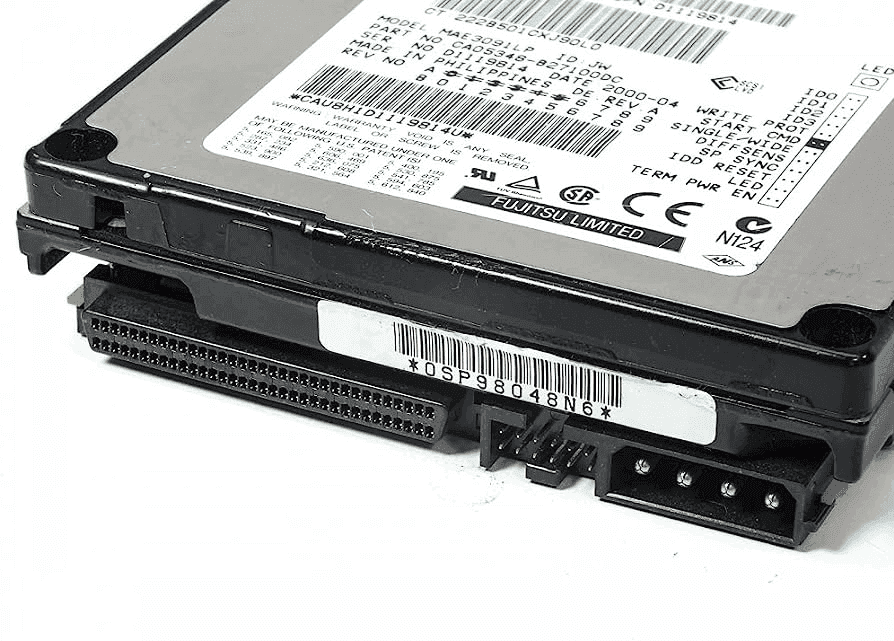
\includegraphics[width=1\linewidth]{extrahovane_obrazky/scsi_hdd.png}
	\end{columns}
	
\end{frame}

\section{SATA}
\begin{frame}{Serial ATA (SATA)}
	\begin{itemize}
		\item Díky pokrokům v metodě přenosu dat nazvané diferential signalling (diferenciální datový pár) bylo možné zvýšit operační frekvenci rozhraní tak, aby dovolilo přenášet dostatečné množství dat sériovým způsobem 
		\item malé úrovně napětí 250 mV
		\item SATA - 1bit šířka, frekvence 1500 MHz - 1,5 Gbit/s.
		\item kódování - 10 bitové
		      \begin{itemize}
		      	\item 150 MB/s (1,5 Gb/s) 
		      	\item 300 MB/s (3 Gb/s) 
		      \end{itemize}
		\item obousměrný přenos (full-duplex)
		\item 4 datové vodiče (Data A+, Data A-, Data B+, Data B-)
		\item 2 stíněné svazky se 2 žilami (4 vodiče dohromady)
	\end{itemize}
\end{frame}


\begin{frame}{Verze SATA}
	\begin{table}[]
		\begin{tabular}{|l|l|l|}
			\hline
			\textbf{přenosový režim} & \textbf{maximální rychlost} & \textbf{standard} \\ \hline
			\textbf{SATA 1}             & 150 MB/s                      & SATA/150          \\ \hline
			\textbf{SATA 2}             & 300 MB/s                      & SATA/300          \\ \hline
			\textbf{SATA 3}             & 600 MB/s                      & SATA/600          \\ \hline
			\textbf{SATA II }           & 3Gb/s                         & SATA 3Gb/s        \\ \hline
		\end{tabular}
	\end{table}
\end{frame}


\begin{frame}{Konektory Serial ATA}
	1. Zem, 2. DATA A+, 3. DATA A-, 4. Zem, \\5. DATA B+, 6. DATA B-, 7. Zem
	
	\begin{columns}
		\column{0.39\textwidth}
		\begin{center}
			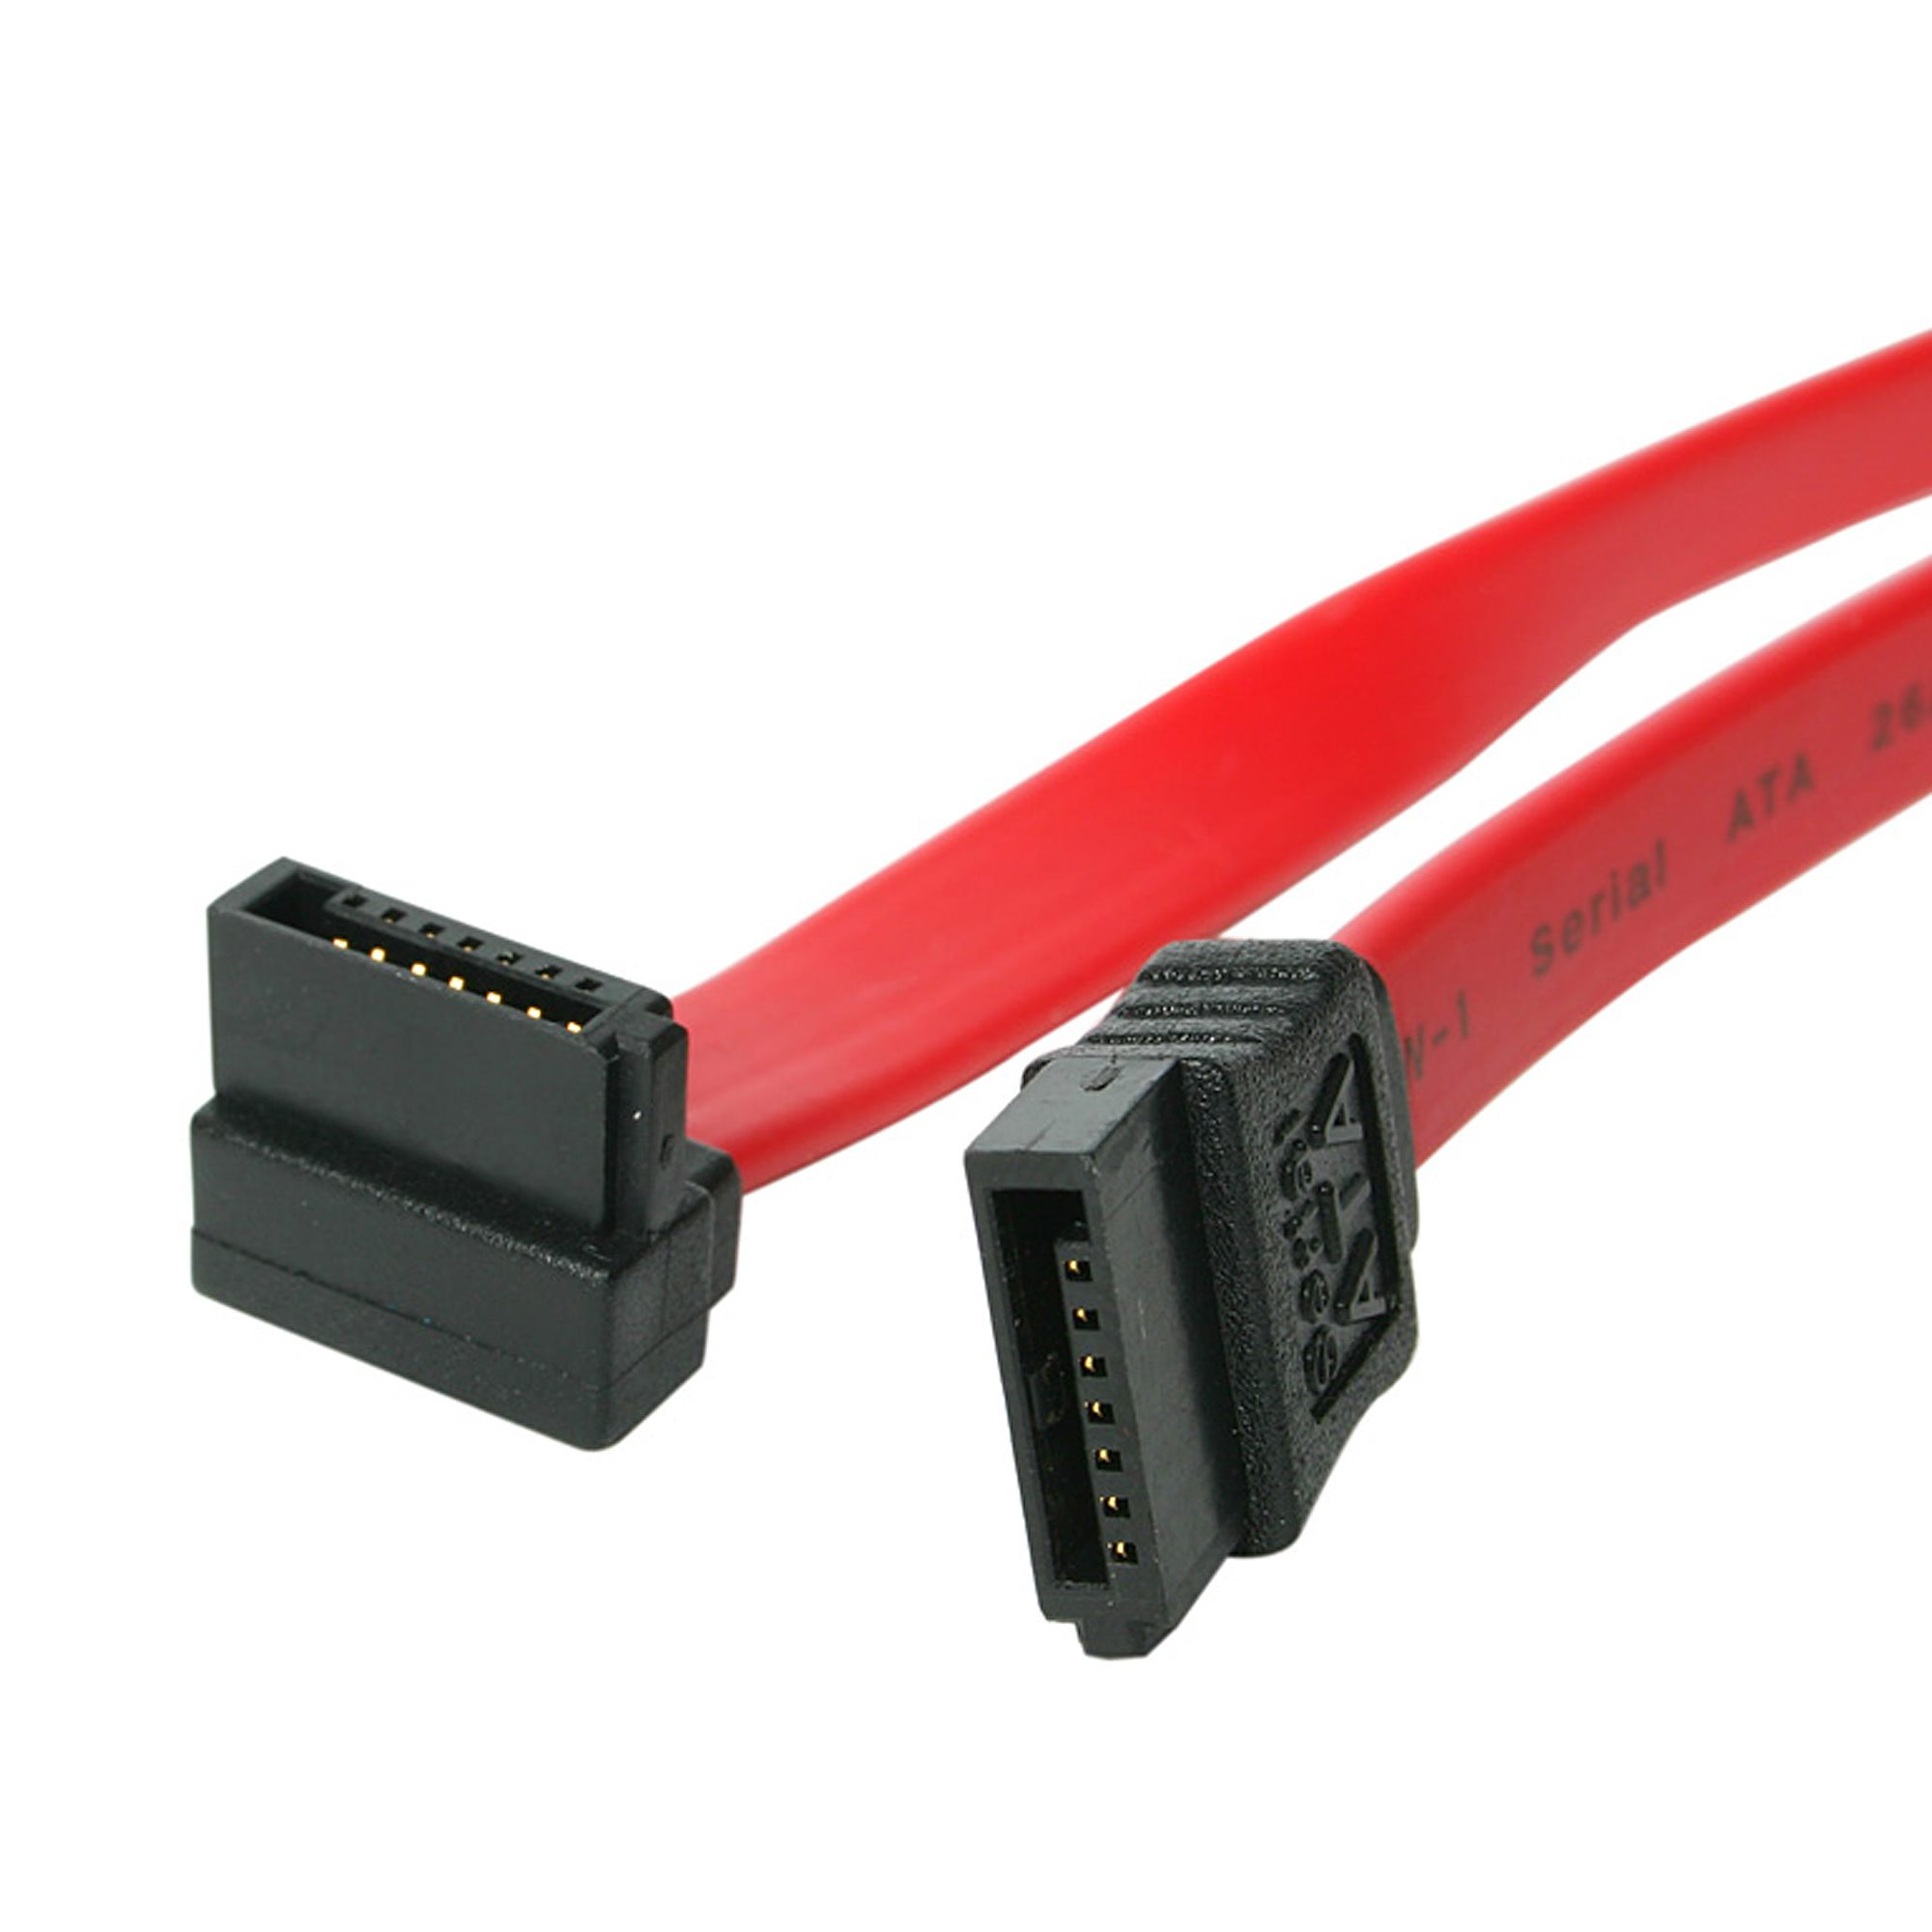
\includegraphics[width=0.8\linewidth]{extrahovane_obrazky/sata_c.jpeg}
		\end{center}
		\column{0.59\textwidth}
		\begin{center}
			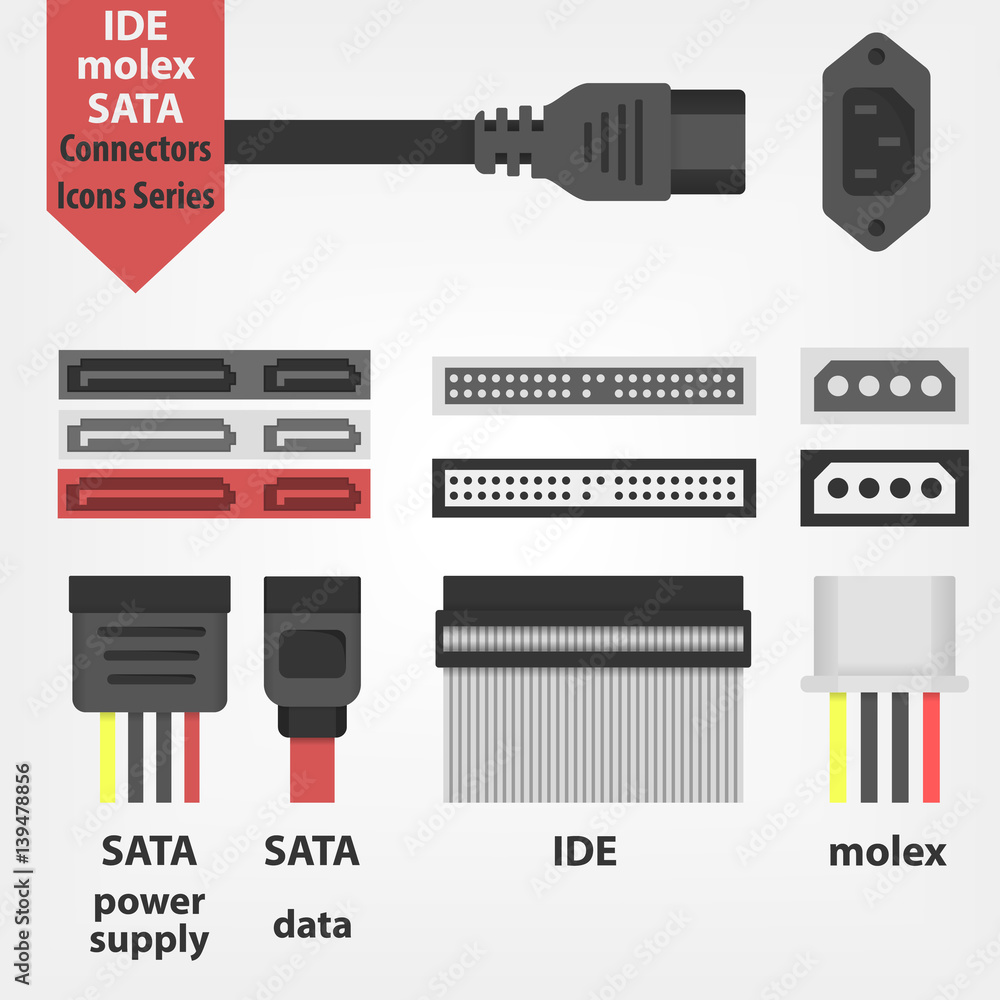
\includegraphics[width=1\linewidth]{extrahovane_obrazky/sata_comp.jpeg}
		\end{center}
	\end{columns}
\end{frame}

\begin{frame}{Redukce IDE - SATA}
	\begin{center}
			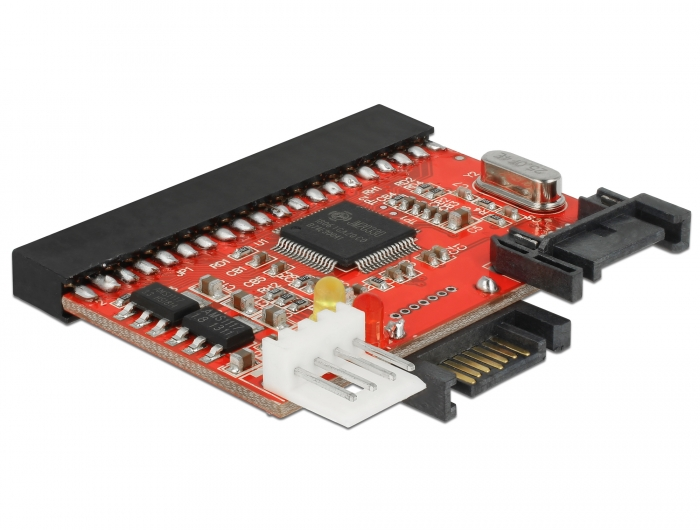
\includegraphics[width=1\linewidth]{extrahovane_obrazky/ide_sata.jpeg}
		\end{center}
\end{frame}


\begin{frame}{Rozdíly mezi SATA-1 a SATA-2 a 3 - AHCI}
	\begin{itemize}
		\item \textbf{Hot-Swap} - dovoluje připojit a odpojit disk za běhu  počítače tak, aby je operační systém rozpoznal
		\item \textbf{Staggered Spin Up} - dokáže po startu počítače minimalizovat energetické nároky na zdroj. Dokáže řídit a ovládat postupný náběh všech pevných disků, které se tak nemusí rozběhnout všechny najednou
		\item \textbf{Port Selecto}r - umožňuje připojit dva řadiče k jednomu disku kvůli zamezení výpadku v případě poruchy jednoho z nich
	\end{itemize}
	
\end{frame}


\begin{frame}{SATA - 2 a 3}
	\textbf{Port Multiplier} slouží k tomu, abychom mohli s jedním řadičem obsloužit více pevných disků, řadiče jsou podstatně rychlejší, než plotnové HDD
	\centering
    \resizebox{0.9\paperwidth}{!}{%
    \begin{tikzpicture}[
        % Define styles for different components
        box/.style={
            draw,
            rectangle,
            minimum width=2cm,
            minimum height=0.8cm,
            thick,
            rounded corners
        },
        controller/.style={
            box,
            fill=pink!20
        },
        multiplier/.style={
            box,
            fill=green!10
        },
        device/.style={
            box,
            fill=blue!10
        },
        arrow/.style={
            ->,
            >=latex,
            thick
        }
    ]

    % Place SATA Host Controller
    \node[controller] (host) {SATA Host\\Controller};

    % Place Port Multiplier
    \node[multiplier, right=2cm of host] (pm) {Port Multiplier};

    % Place SATA devices
    \foreach \i in {1,...,5} {
        \node[device, right=2cm of pm] (dev\i) at ([yshift=2-\i cm]pm.east) {SATA Device \i};
    }

    % Draw connections with speed labels
    \draw[arrow] (host) -- node[above] {6.0 Gb/s} (pm);
    \foreach \i in {1,...,5} {
        \draw[arrow] (pm) -- node[above] {6.0 Gb/s} (dev\i);
    }

    \end{tikzpicture}
    }
	
\end{frame}


\begin{frame}{Technologie NCQ (Native Command Queuing)}
	Přirozené řazení požadavků. Technologie ponechává rozhodování o pořádí čtení dat na logice disku a posloupnost čtení dat si seřadí tak, aby k tomu potřeboval co nejméně otáček a přesunů hlavy.
	\begin{center}
		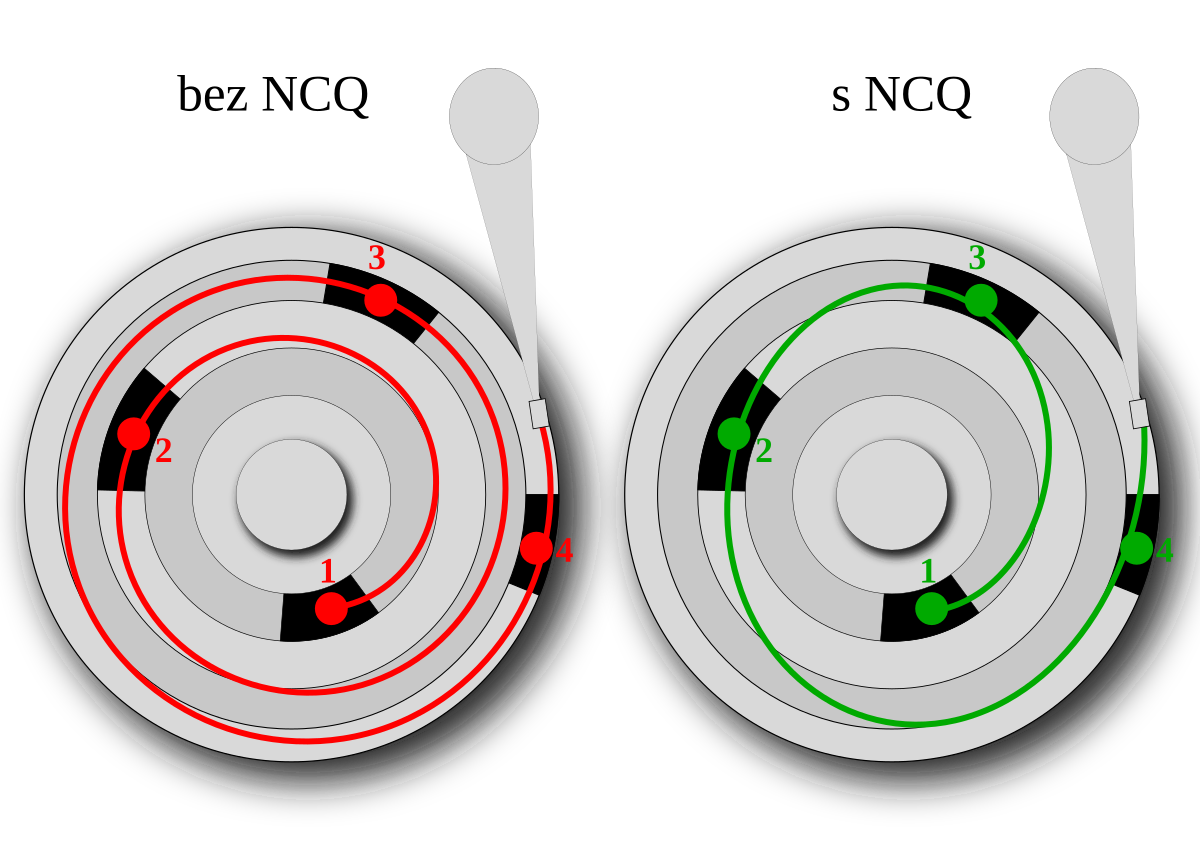
\includegraphics[width=0.8\linewidth]{extrahovane_obrazky/ncq.png}
	\end{center}
	
\end{frame}


\begin{frame}{eSATA (External SATA)}
	\begin{itemize}
		\item Během probíhajícího přenosu zatěžuje procesor zcela minimálně (daleko méně než např. USB). 
		\item Narozdíl od externích disků s rozhraním USB 2.0 nebo IEEE1394 FireWire dokáže poskytnout plný výkon SATA a také podporu SMART.
		\item eSATA kabel -> eSATA konektor v počítači -> normální datový SATA kabel
		\item Má lépe zpracovaný konektor kvůli častému připojování a odpojování disku (Hot Plug) 
		\item konstrukčně až na 500 zasunutí, ( SATA - 50 zasunutí)
		\item délka kabelu až 2 m
	\end{itemize}
\end{frame}


\begin{frame}{Konektory eSATA}
\begin{center}
			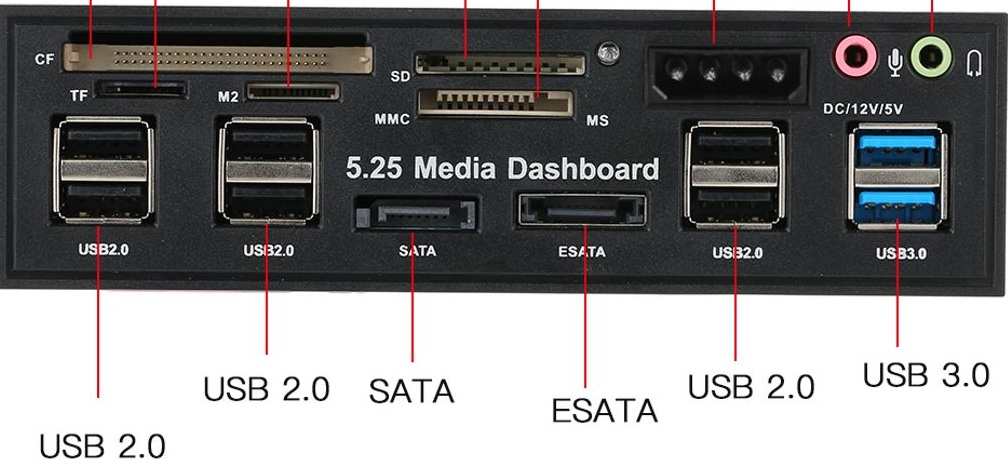
\includegraphics[width=0.6\linewidth]{extrahovane_obrazky/esata.jpg}
		\end{center}
        \begin{center}
			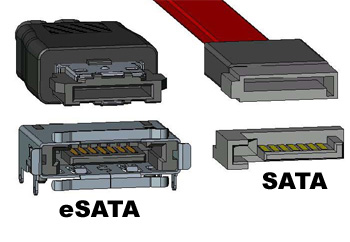
\includegraphics[width=0.5\linewidth]{extrahovane_obrazky/sata_esata.jpeg}
		\end{center}
	
\end{frame}


\begin{frame}{mSATA (mini SATA)}
	Konektor mSATA a Mini PCI Express je stejný a o tom co podporuje 
	rozhoduje firmware.
	\begin{center}
		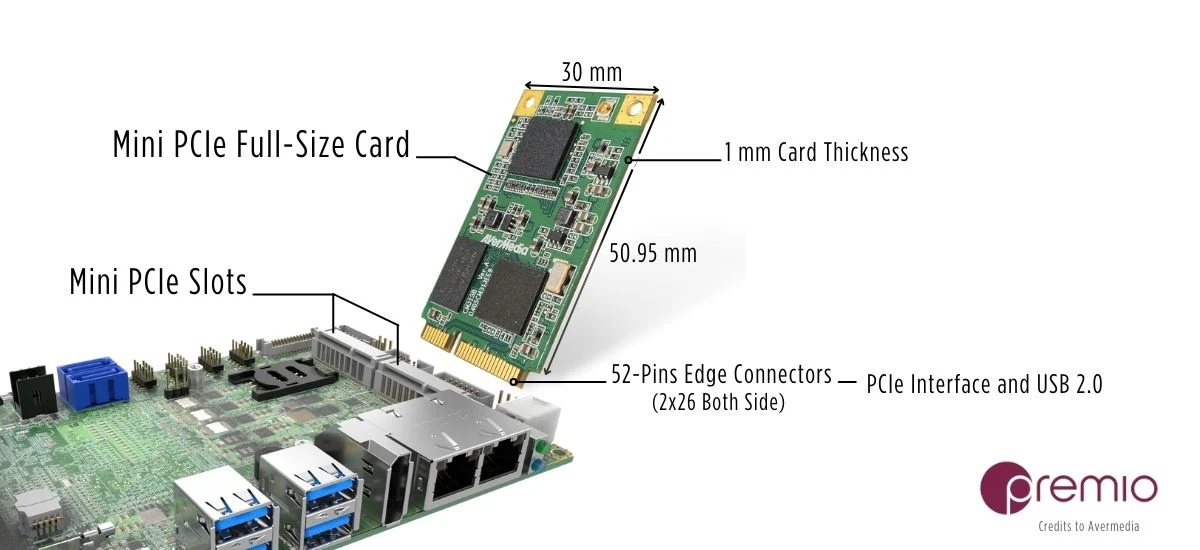
\includegraphics[width=1\linewidth]{extrahovane_obrazky/mpcie.jpg}
	\end{center}
	
\end{frame}

\begin{frame}{mSATA}
	 
	\begin{center}
		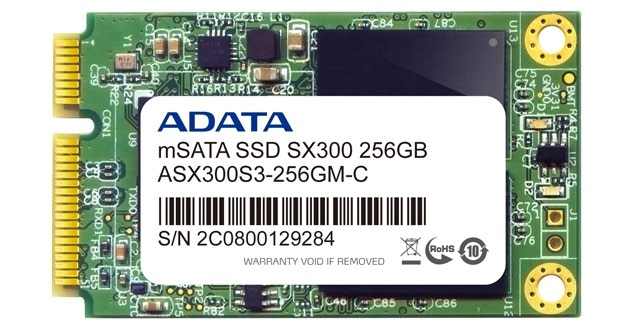
\includegraphics[width=1\linewidth]{extrahovane_obrazky/img_2_page15_0.jpeg}
	\end{center}
\end{frame}


\begin{frame}{SATA Express (2013)}
	\begin{center}
		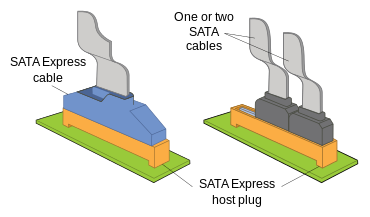
\includegraphics[width=1\linewidth]{extrahovane_obrazky/Sata-Express.png}
	\end{center}
	
\end{frame}


\begin{frame}{SATA Express specifikace}
	\begin{center}
		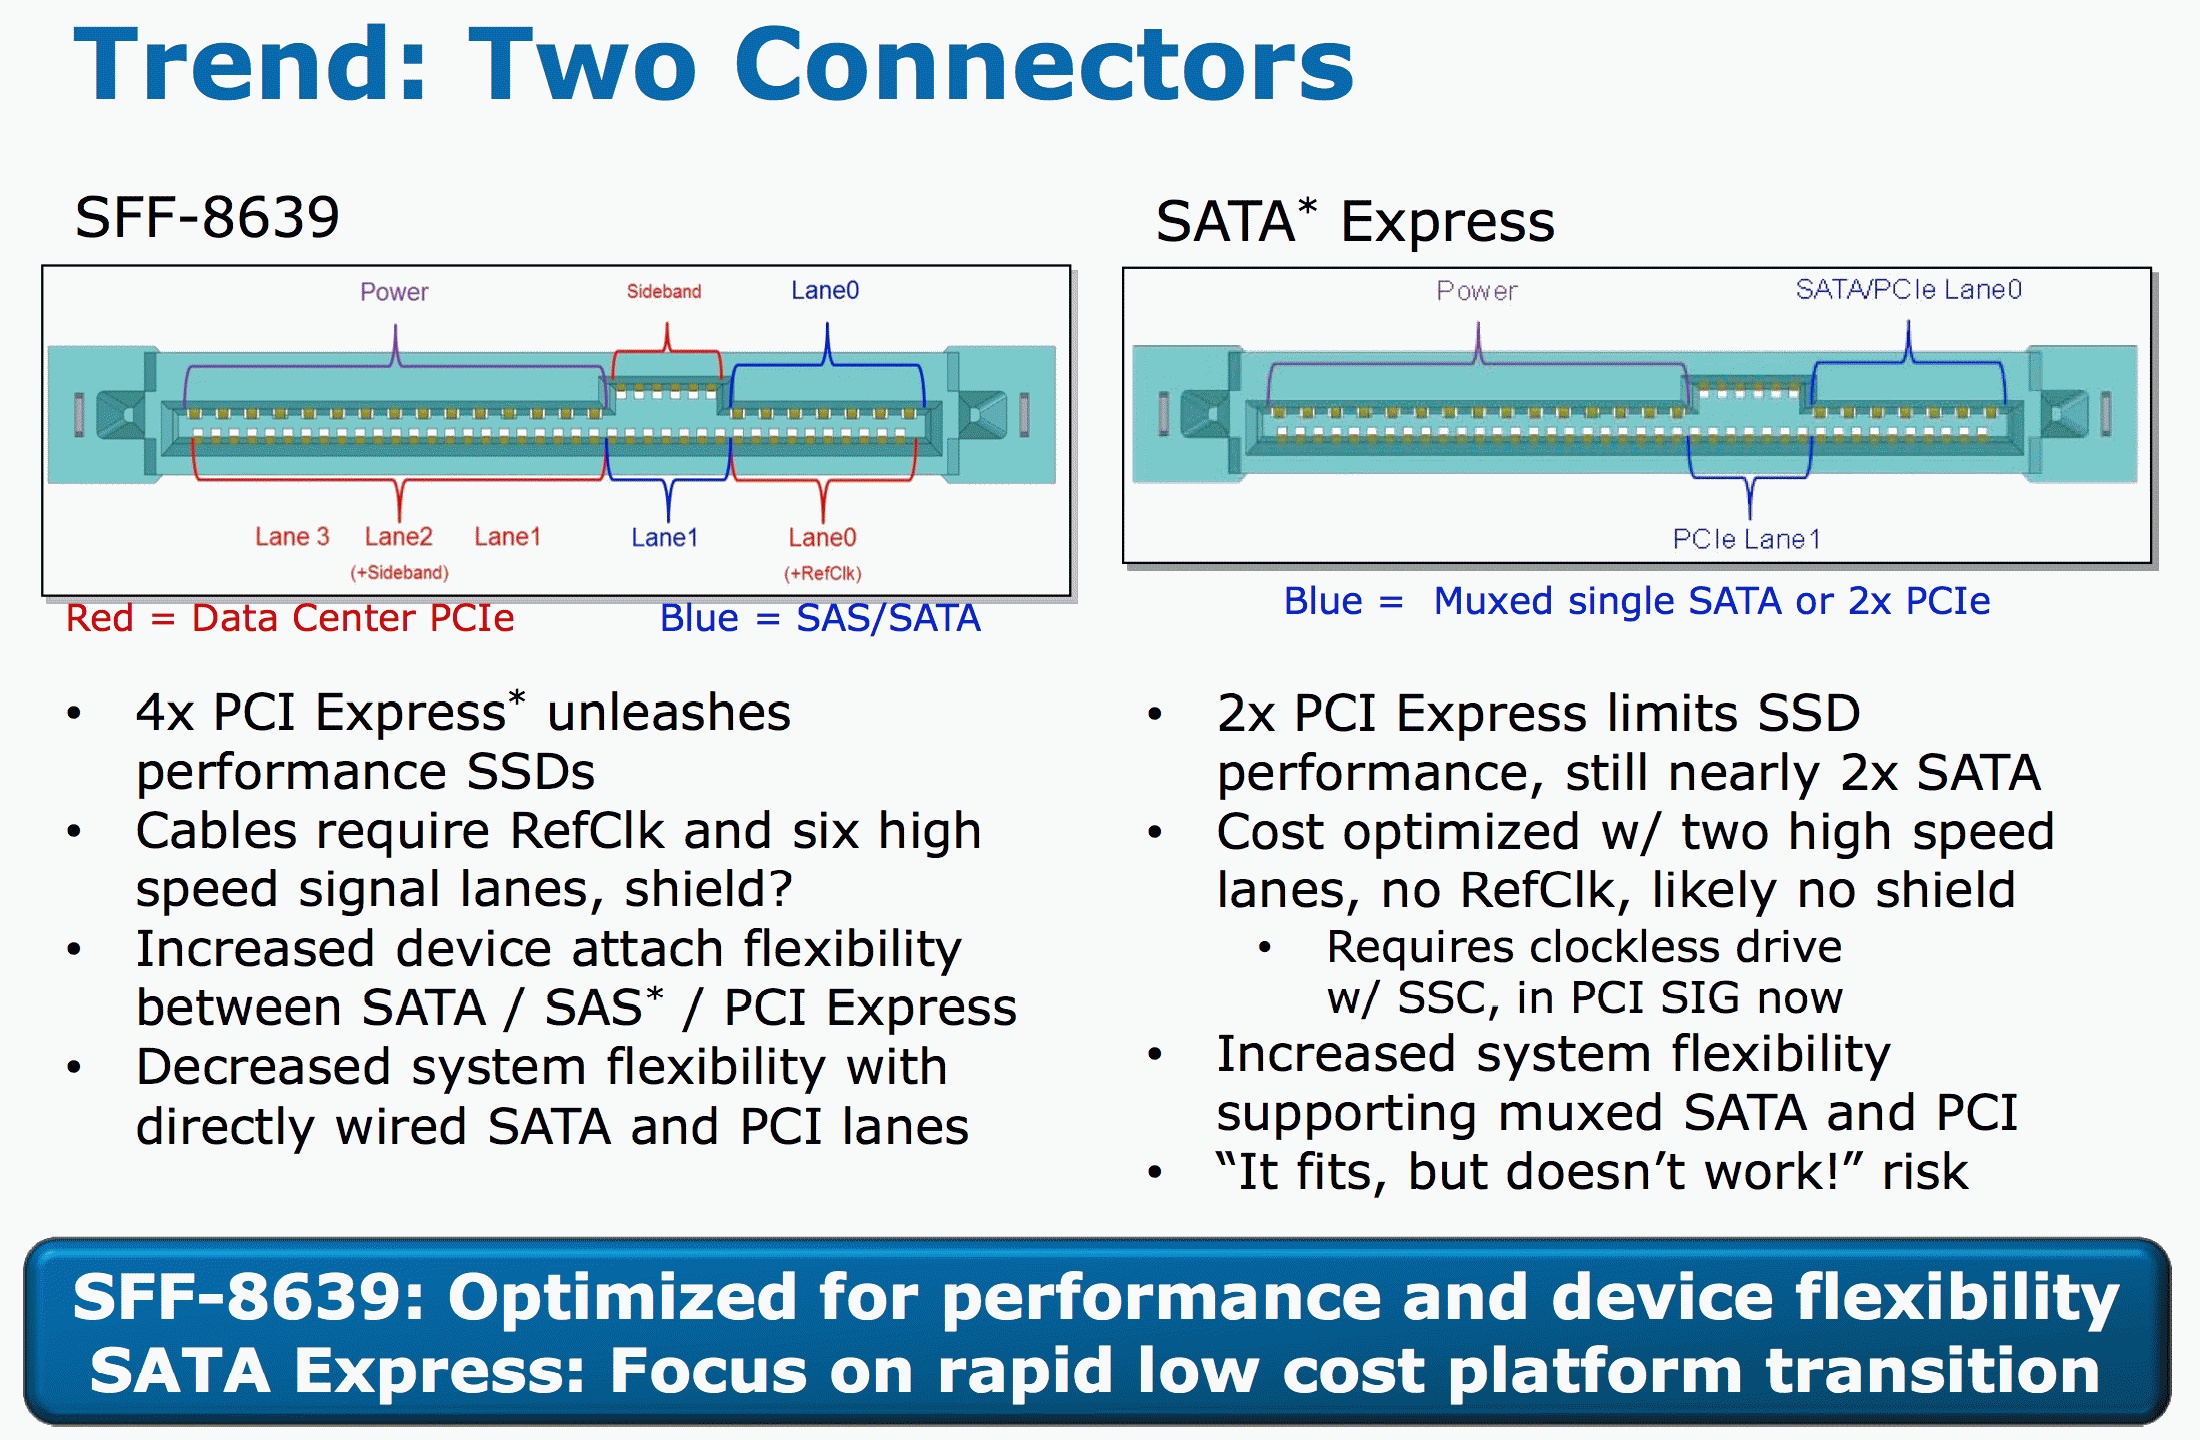
\includegraphics[width=0.8\linewidth]{extrahovane_obrazky/img_2_page17_0.png}
	\end{center}
	
\end{frame}


\begin{frame}{SATA Express}
	 
	\begin{center}
		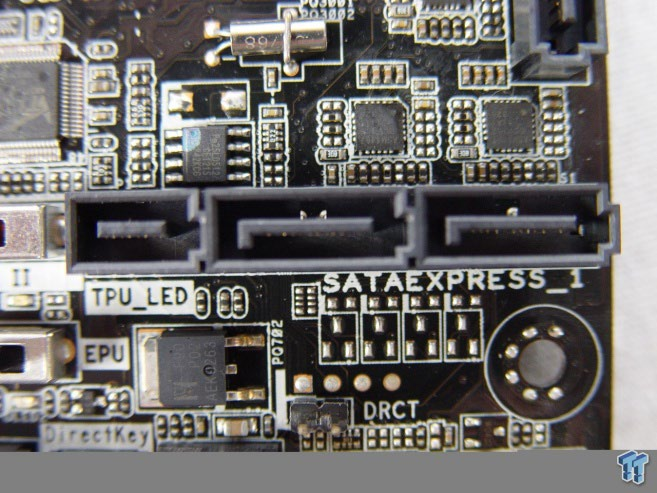
\includegraphics[width=0.8\linewidth]{extrahovane_obrazky/img_2_page18_0.jpeg}
	\end{center}
	
\end{frame}


\begin{frame}{Kabely SATA Express}
	Každý konektor SATA Express v sobě nese dva porty SATA 6 Gb/s a dvě linky PCI-E. Disk pak může komunikovat se systémem buď přes SATA nebo i pomocí PCI-E. 
	Pokud jde komunikace přes PCI-E linky, může klidně probíhat i skrze protokol NVMe, tedy bez AHCI a přímo s procesorem. \\
	Jelikož dvě linky PCI-E jsou málo, od tohoto řešení se ustupuje, nahradil jej slotM.2.
	\begin{center}
		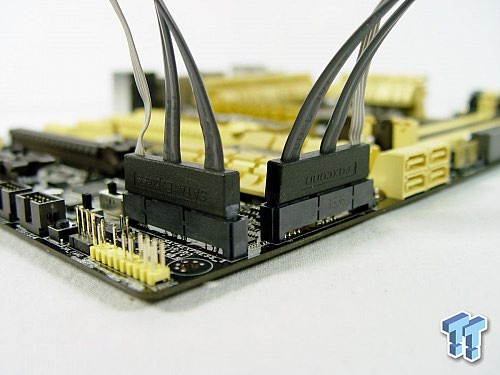
\includegraphics[width=0.6\linewidth]{extrahovane_obrazky/img_2_page19_0.jpeg}
	\end{center}
\end{frame}


\begin{frame}{SATA Express prakticky}
	\begin{center}
		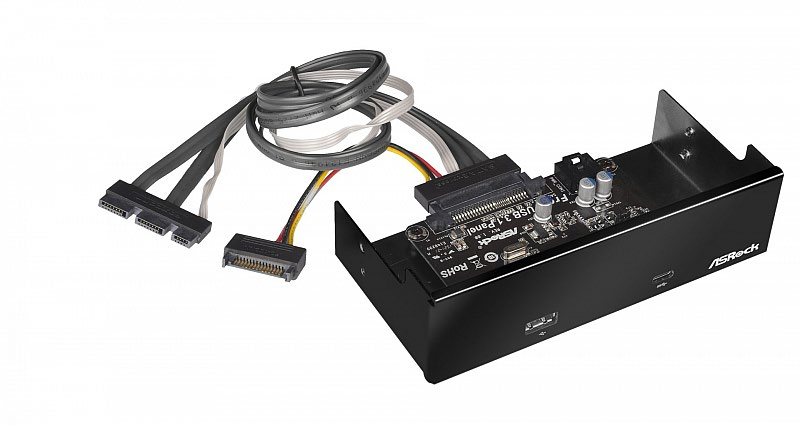
\includegraphics[width=1\linewidth]{extrahovane_obrazky/img_2_page21_0.jpeg}
	\end{center}
	
\end{frame}


\section{NGFF}
\begin{frame}{NGFF}
	nástupce mSATA a SATAe byl nejdříve NGFF a následně M.2
	\begin{center}
		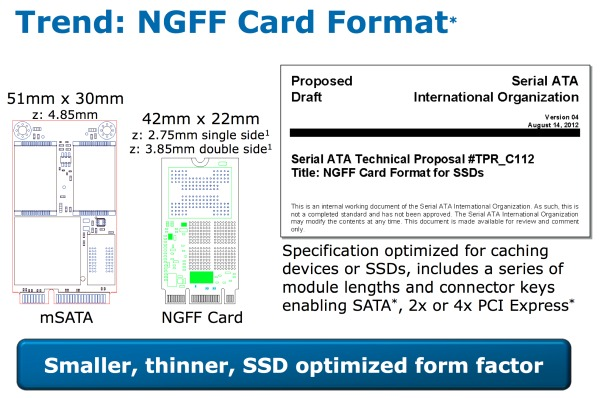
\includegraphics[width=0.8\linewidth]{extrahovane_obrazky/img_2_page22_0.png}
	\end{center}
	
\end{frame}

\section{M.2}
\begin{frame}{mSATA X M.2}
	mSATA nese pouze jedno SATA rozhraní, M.2 může nést v podstatě cokoliv.
	\begin{center}
		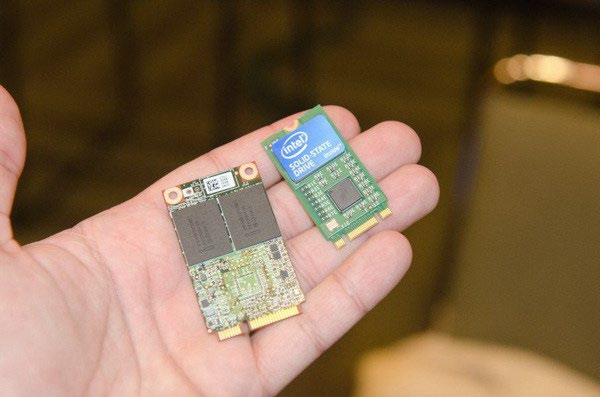
\includegraphics[width=0.9\linewidth]{extrahovane_obrazky/img_2_page23_0.jpeg}
	\end{center}
	
\end{frame}


\begin{frame}{Verze M.2 konektorů}
	\begin{itemize}
		\item Dle specifikace je v jednom M.2 konektoru čtveřice PCI-E linek (2.0, 3.0), dvojice kanálů SATA 6 Gb/s, trojice kanálů USB (2.0, 3.0), PCM Audio a spousta dalších možností. 
		\item M.2 je univerzální konektor, k jehož funkcím je nutné přistupovat klíčováním kontaktů.
		\item „B“. To je klasické SATA Express a něco navíc. Např. dvě PCI-E linky, jeden SATA port, USB kanál, zvuk a další
		\item Pro SSD disky je vhodnější konektor a klíčování „M“. To zabezpečuje připojení čtyř linek PCI-E s jedním SATA portem.
	\end{itemize}
	
	
	\begin{center}
		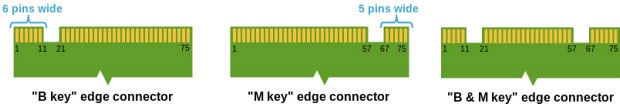
\includegraphics[width=1\linewidth]{extrahovane_obrazky/img_2_page24_0.jpeg}
	\end{center}
	
\end{frame}


\begin{frame}{Porovnání mSATA a verzí M.2}
	 
	\begin{center}
		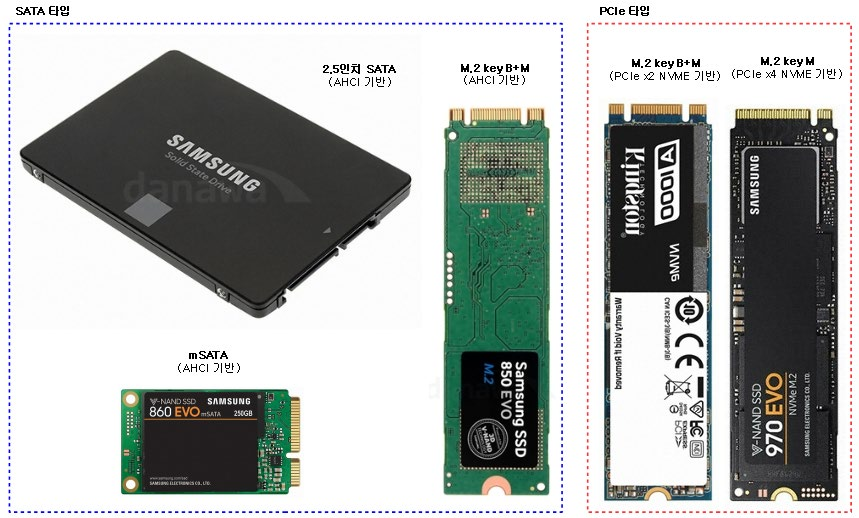
\includegraphics[width=1\linewidth]{extrahovane_obrazky/img_2_page26_0.jpeg}
	\end{center}
	
\end{frame}


\begin{frame}{}
	 
	\begin{center}
		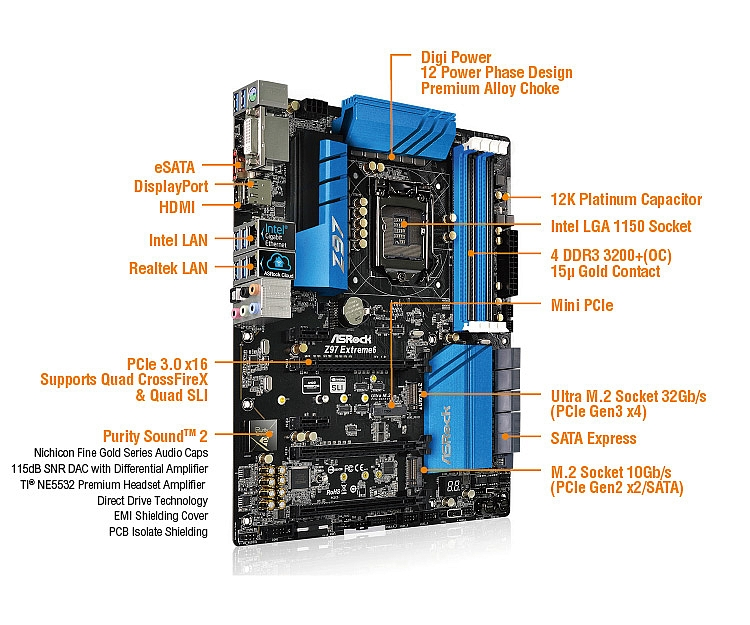
\includegraphics[width=1\linewidth]{extrahovane_obrazky/img_2_page27_0.png}
	\end{center}
	
\end{frame}


\begin{frame}{SFF 8639 – nové označení U.2 - M.2 pro Hot Swap}
	Kabel s konektory miniSAS HD a U.2
	\begin{center}
		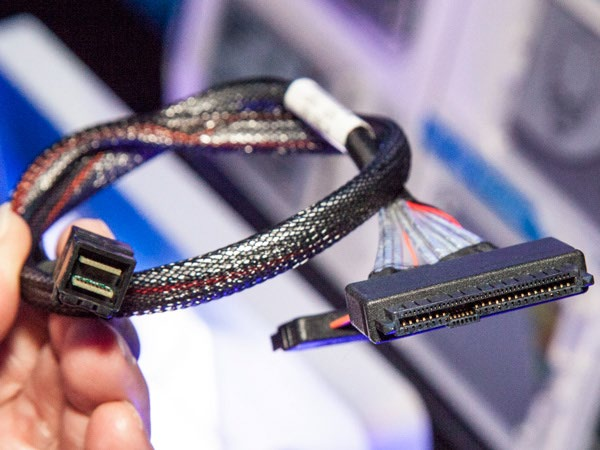
\includegraphics[width=0.8\linewidth]{extrahovane_obrazky/img_2_page28_1.jpeg}
	\end{center}
	
\end{frame}


\begin{frame}{Dnes na verzi PCI- E i na počtu linek záleží}
	 
	\begin{center}
		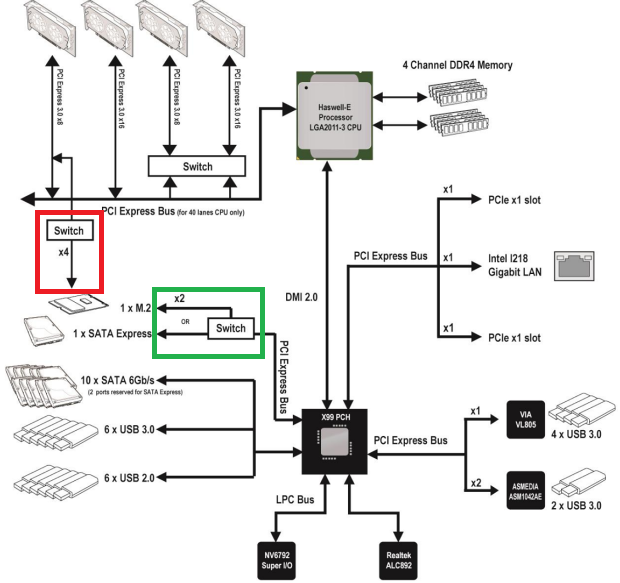
\includegraphics[width=0.8\linewidth]{extrahovane_obrazky/img_2_page29_0.png}
	\end{center}
	
\end{frame}

\section{AHCI}
\begin{frame}{AHCI (Advenced Host Controler Interface)}
	\begin{itemize}
		\item AHCI (Advenced Host Controler Interface) je hardwarová vrstva mezi čipsetem a SATA zařízením, nachází se na úrovni PCI rozhraní. Jeho hlavním účelem je umožnit komunikaci mezi software a SATA disky či mechanikami na úrovni, kterou PATA řadiče již nedokáží. 
		\item Pokročilé funkce jako je hot-plugging nebo NCQ. Působí jako „urychlovač a překladač datových požadavků.
		\item Eliminace rozdělení disků na Master a Slave, 64bitové adresování, ovládání stavových LED, power managing, port multiplier
	\end{itemize}
	
\end{frame}


\begin{frame}{AHCI HBA (Host Bus Controler)}
	Většina nativních SATA řadičů umožňuje práci ve třech režimech – legacy, čili IDE kompatibilní, druhým je povolení AHCI, které při osazení počítače jediným diskem umožní nejsnazší využívání hot-plugu nebo NCQ, a nakonec možnost zapojení do RAID (nejčastěji 1,0 se dvěma nebo 5 se čtyřmi disky).
	\\
	Intel doporučuje bez závislosti na osazení disky používat RAID mód, který v případě detekce jediného disku nijak nezasahuje do práce systému, ale váš počítač je kdykoli připraven na další rozšíření.
	
\end{frame}

\section{NVMe}
\begin{frame}{Co znamená NVMe}
	\textbf{Non-Volatile Memory Host Controller Interface}
	\begin{itemize}
		\item AHCI - rok 2004, pevné disky s mechanickým ukládaním dat
		\item Tmavě modrá - latence pevného disku (přístupová doba, rychlost řadiče, odezva disku)
		\item Fialová - zpoždění v diskovém řadiči (zpravidla čip na desce nebo obvody v čipsetu)
		\item Světle a tmavě zelená - reakční doba softwaru, neboli ovladače.
	\end{itemize}
	\begin{center}
		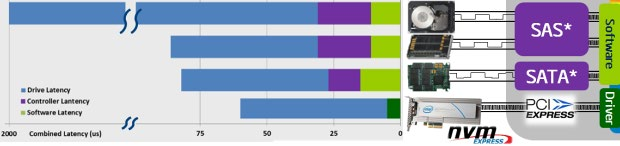
\includegraphics[width=1\linewidth]{extrahovane_obrazky/img_2_page32_1.jpeg}
	\end{center}
	
\end{frame}


\begin{frame}{NVMe jaký je teda rozdíl?}
	\begin{itemize}
		\item mechanicky disk - latence v tisících mikrosekund
		\item SSD na AHCI - latence 80 mikrosekund (řadič a ovladač)
		\item NVMe protokol - procesor komunikuje s diskem přímo, nepotřebuje k tomu žádný řadič - latence 60 mikrosekund
		\item výsledek? - sedmkrát narostla přenosová kapacita a třikrát se snížila latence
	\end{itemize}
	
	\begin{center}
		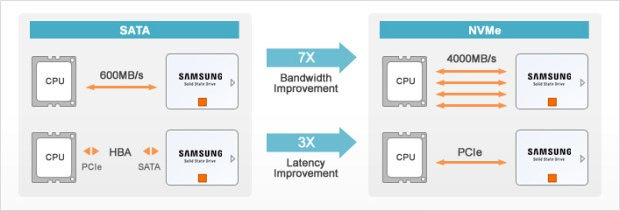
\includegraphics[width=1\linewidth]{extrahovane_obrazky/img_2_page33_0.jpeg}
	\end{center}
	
\end{frame}


\begin{frame}{NVMe prakticky}
	AHCI fronta pro 1 milion IOPS potřebuje deset procesorových jader, procesory potřebují ke zpracování 27 tisíc cyklů a trvá to deset mikrosekund. Ta stejná úloha, u NVMe zatíží pouze necelá 
	čtyři procesorová jádra, zpracování zabere procesorům 10 tisíc cyklů a pouze tři mikrosekundy. Zátěž procesoru je nižší, zpracování požadavků rychlejší.
	\begin{center}
		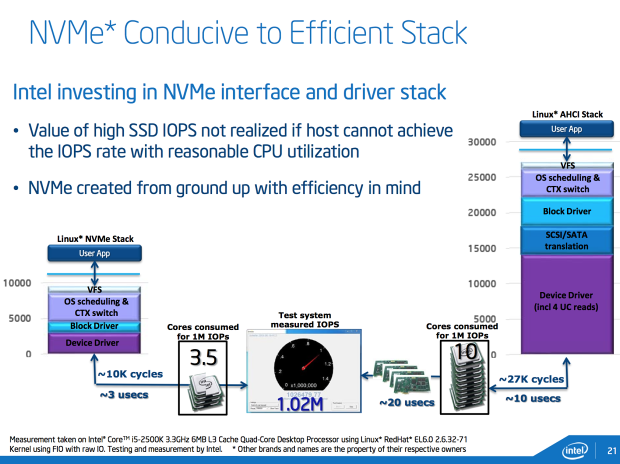
\includegraphics[width=0.6\linewidth]{extrahovane_obrazky/img_2_page34_0.png}
	\end{center}
	
\end{frame}


\begin{frame}{NVMe - závěr}
	\begin{itemize}
		\item technologie pro SSD disky připojené k PCI-E rozhraní
		\item Disk komunikuje s procesorem přímo (pokud jsou PCI-E linky přímo v něm, jako u Intelu. )Není potřeba žádný řadič, jen ovladač v systému. Přístupová doba je značně kratší a propustnost až 8GB/s (jedním směrem) při použití osmi PCI-E 3.0 linek.
		\item U AHCI je daná jen jedna příkazová fronta s třiceti dvěma příkazy, u NVMe je front 64 tisíc a každá se 64 tisíci příkazy najednou. NVMe podporuje vícenásobný přístup, a paralelizaci na straně procesoru. Počet IOPS není limitován jedním jádrem procesoru, lze využít všechna jádra.
	\end{itemize}
	
	\begin{center}
		
\includegraphics[width=0.6\linewidth]{extrahovane_obrazky/img_2_page35_0.jpeg}
	\end{center}
	
\end{frame}


\begin{frame}{NVMe M.2 (vpravo) a SATA M.2 (vlevo)}
	SATA disky mají zářezy dva, NVMe mají jen jeden, což znamená určitou míru kompatibility. Pokud je M.2 slot NVMe kompatibilní, je velká šance, že v něm budou fungovat také SATA SSD, opačně to však vzhledem k povaze socketů neplatí. Je zároveň možné, že slot kompatibilní nebude, případně bude potřeba režim M.2 slotu ručně nastavit 
	v BIOSu. Ve všech situacích je však dobré si předem 
	kompatibilitu ošetřit a zkontrolovat, zda základní deska 
	disponuje správným rozhraním.\\
    nová M.2 - PCIe 5.0 M.2 SSD, které dosahují rychlostí až 14 GB/s
	
	\begin{columns}
		\column{0.49\textwidth}
		\begin{center}
			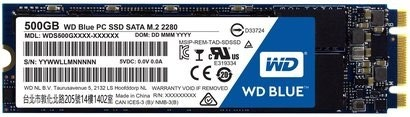
\includegraphics[width=1\linewidth]{extrahovane_obrazky/img_2_page36_0.jpeg}
		\end{center}
		\column{0.49\textwidth}
		\begin{center}
			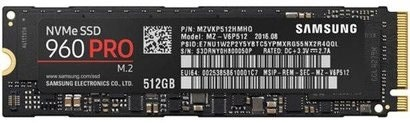
\includegraphics[width=1\linewidth]{extrahovane_obrazky/img_2_page36_1.jpeg}
		\end{center}
	\end{columns}
\end{frame}

\section{SAS}
\begin{frame}{\textbf{SAS} (Serial Attached SCSI)}
	pokračovatel SCSI rozhraní,  v sériovém provedení, 
	používá se u nejvýkonnějších serverových disků s 
	rychlostmi otáčení ploten až 15~000 rpm. Konektor 
	podobný SATA
	\begin{center}
		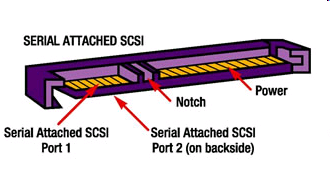
\includegraphics[width=0.8\linewidth]{extrahovane_obrazky/img_2_page37_0.png}
	\end{center}
	Hitachi GST (2012) disk se SAS 12Gb/s - 2 porty -> 4,8 GB/s
\end{frame}

\section{FireWire}
\begin{frame}{FireWire - IEEE1394}
	vysokorychlostní sériová sběrnice (peer to peer) vyvinutá společností Apple sloužící k připojení externích disků, rychlost dnes až 800 Mb/s (100 MB/s) (2007), pracuje se na 6,4 Gb/s (teď už ne - nástupce Thunderbolt)
	
	\begin{center}
		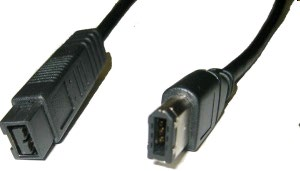
\includegraphics[width=0.8\linewidth]{extrahovane_obrazky/img_2_page39_0.jpeg}
	\end{center}
	
\end{frame}

\section{Rozraní USB}
\begin{frame}{Rozhraní USB}
	\begin{itemize}
		\item sériové rozhraní
		\item rychlost 1.5, 12, 480 Mb/s, 4.8Gb/s
		\item připojení zařízení až na vzdálenost 5 m
		\item možnost napájení z konektoru
		\item až 127 připojených zařízení
		\item podpora plug \& play
		\item topologie založená na USB rozbočovačích (HUB), které zároveň pracují jako opakovače (repeater – zesiluje signál)
	\end{itemize}
	
	
\end{frame}


\begin{frame}{Architektura}
	\begin{itemize}
		\item max. 7 hubů, max. 127 zařízení
	\end{itemize}
	\begin{center}
		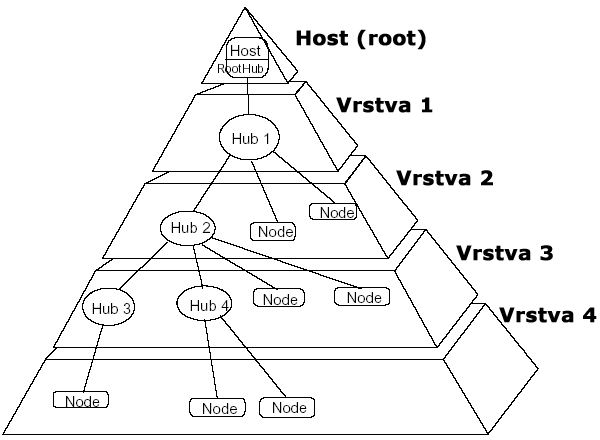
\includegraphics[width=0.8\linewidth]{extrahovane_obrazky/img_3_page2_0.png}
	\end{center}
	
\end{frame}


\begin{frame}{Konektory}
	\begin{columns}
		\column{0.49\textwidth}
		\begin{center}
			Typ A
			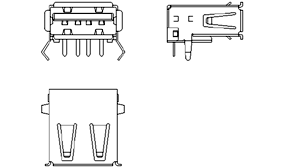
\includegraphics[width=0.9\linewidth]{extrahovane_obrazky/img_3_page3_1.png}
			Typ B
			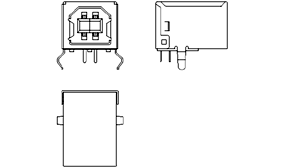
\includegraphics[width=0.9\linewidth]{extrahovane_obrazky/img_3_page3_2.png}
		\end{center}
		\column{0.49\textwidth}
		\begin{center}
			Typ „mini“
			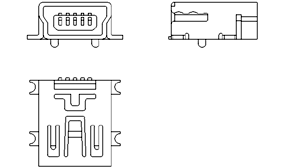
\includegraphics[width=1\linewidth]{extrahovane_obrazky/img_3_page3_3.png}
		\end{center}
	\end{columns}
	
\end{frame}

\begin{frame}{Vývody konektoru}
	\begin{table}
		\begin{tabular}{|l|l|l|}
			\hline
			\textbf{Číslo vývodu} & \textbf{Význam} & \textbf{Barva}             \\ \hline
			1                        & +5 V             & \textcolor{red}{červená} \\ \hline
			2                        & Data --          & \textcolor{black}{bílá}  \\ \hline
			3                        & Data +           & \textcolor{green}{zelená} \\ \hline
			4                        & GND              & černá                    \\ \hline
		\end{tabular}
	\end{table}
	
	\begin{columns}
		\column{0.49\textwidth}
		\begin{center}
			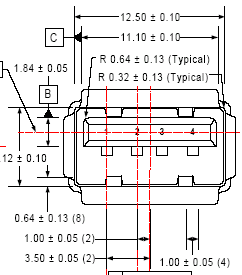
\includegraphics[width=0.7\linewidth]{extrahovane_obrazky/img_3_page4_9.png}
		\end{center}
		\column{0.49\textwidth}
		\begin{center}
			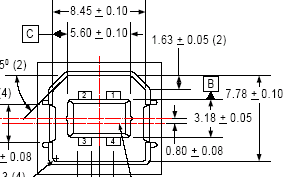
\includegraphics[width=1\linewidth]{extrahovane_obrazky/img_3_page4_10.png}
		\end{center}
	\end{columns}
\end{frame}


\begin{frame}{USB kabel}
	\begin{itemize}
		\item stíněný nebo nestíněný (pro Low Speed, max. délka 3 metry)
		\item data - kroucený pár, napájení - napřímo
		\item stínění je připojeno jen na straně počítače k pinu GND, zařízení ho již nepřipojuje
	\end{itemize}
	\begin{center}
		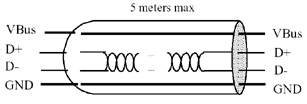
\includegraphics[width=0.8\linewidth]{extrahovane_obrazky/img_3_page5_0.png}
	\end{center}
	
\end{frame}


\begin{frame}{Verze USB}
	\begin{itemize}
		\item 1.1 – teoretická propustnost max. 12 Mb/s
		\item 2.0 – teoretická propustnost max. 480 Mb/s
		\item 3.0 - Super Speed - teoretická propustnost  max. 4.8 Gb/s (600 MB/s), 
		      \begin{itemize}
		      	\item 8 vodičů (6 datových + 2 napájecí)
		      \end{itemize}
	\end{itemize}
	Rychlost je závislá na limitech technologie, množství Hubů na cestě, délce kabelu a konstrukci samotného zařízení.\\
	Reálná přenosová rychlost bývá sotva poloviční (2.0 – 30 MB/s, 3.0 – 60 MB/s)
	
	\begin{table}
		\begin{tabular}{|l|l|}
			\hline
			\begin{tabular}[c]{@{}l@{}}Low &                                     \\Speed\end{tabular} & 1.5 Mb/s \\ \hline
			Full Speed                     & 12 Mb/s                             \\ \hline
			High Speed                     & \begin{tabular}[c]{@{}l@{}}480 Mb/s \\(60 MB/s)\end{tabular} \\ \hline
		\end{tabular}
	\end{table}
	
\end{frame}


\begin{frame}{Definice rychlosti zařízení}
	\begin{itemize}
		\item Zařízení mohou být připojena za chodu, je třeba jejich zařízení rozpoznat a určit rychlost, s jakou jsou schopna komunikovat.
		\item Řešení: změna napětí na některém z datových vodičů.
		\item Zařízení USB 1.1 nemusí podporovat Full Speed
	\end{itemize}
	
	\begin{columns}
		\column{0.49\textwidth}
		\begin{center}
			Low Speed
			\includegraphics[width=1\linewidth]{extrahovane_obrazky/img_3_page7_4.png}
		\end{center}
		\column{0.49\textwidth}
		\begin{center}
			Full Speed
			\includegraphics[width=1\linewidth]{extrahovane_obrazky/img_3_page7_5.png}
		\end{center}
	\end{columns}
	
\end{frame}


\begin{frame}{High Speed}
	\begin{itemize}
		\item Zapojeno stejně jako Full Speed 
		\item Ze začátku také tak komunikuje na FS, zvýšení rychlosti je 
		      potom řešeno softwarově.
		\item Zařízení USB 2.0 nemusí podporovat High Speed
	\end{itemize}
	
\end{frame}


\begin{frame}{Přenos dat}
	\begin{itemize}
		\item není přenášen hodinový signál, synchronizace na základě dat
		\item kódování NRZI (Non Return to Zero Invert)
		      \begin{itemize}
		      	\item 0 – změna úrovně, 1 - ponechání úrovně
		      	\item sync-byte 00000001
		      \end{itemize}
		\item bit stuffing - vynucení změny
		      \begin{itemize}
		      	\item po každých 6-ti jedničkách vložena nula, příjemce nuly navíc odstraňuje
		      	\item paket obsahující víc než 6 jedniček za sebou je  ignorován
		      \end{itemize}
		\item datové vodiče přenáší vzájemně negovaný signál
	\end{itemize}
	
	
	\begin{center}
		\includegraphics[width=1\linewidth]{extrahovane_obrazky/NRZI.png}
	\end{center}
\end{frame}



\begin{frame}{Napájení z USB - standardy}
	\begin{itemize}
		\item hub dodává 4.75 – 5.25 V, max. pokles o 0.35 V
		\item zařízení odebírá max. 100 mA, zařízení může specifikovat, že potřebuje méně
		\item zařízení může požádat až o 500 mA (nedojde-li k poklesu)
		\item hub napájený po sběrnici je schopen dodávat max. 100~mA~/~port
		\item USB 3.0 – max. 900 mA
		      \begin{itemize}
		      	\item vylepšená správa napájení
		      	\item existují 3 úsporné režimy
		      \end{itemize}
	\end{itemize}
\end{frame}


\begin{frame}{Organizace sběrnice}
	\begin{itemize}
		\item one-master - většinou počítač, veškerá aktivita vychází od něj
		\item zařízení může zahájit přenos jen po vyzvání
		\item 1.0 a 2.0 – poloviční duplex
		\item 3.0 – plný duplex – lze komunikovat v obou směrech současně
	\end{itemize}
\end{frame}


\begin{frame}{USB 3.0}
	Na rozdíl od USB 2.0 přibyly dva diferenciální páry - SSTX (+/-) -
	twistovaný pár pro Super Speed (USB 3.0) ve směru vysílání a SSRX 
	(+/-) - twistovaný pár pro Super Speed (USB 3.0) ve směru příjmu.\\
	Dva vodiče D(+/-) slouží pro zpětnou kompatibilitu s USB 2.0 
	(standardní USB 2.0 sběrnice). Zbylé dva vodiče jsou napájecí.
	
	\begin{columns}
		\column{0.49\textwidth}
		\begin{center}
			\includegraphics[width=1\linewidth]{extrahovane_obrazky/img_3_page14_0.jpeg}
		\end{center}
		\column{0.49\textwidth}
		\begin{center}
			\includegraphics[width=1\linewidth]{extrahovane_obrazky/img_3_page14_1.jpeg}
		\end{center}
	\end{columns}
	
\end{frame}


\begin{frame}{USB – 3.0}
	
	\begin{columns}
		\column{0.49\textwidth}
		\begin{center}
			\includegraphics[width=1\linewidth]{extrahovane_obrazky/img_3_page15_1.jpeg}
		\end{center}
		\column{0.49\textwidth}
		\begin{center}
			\includegraphics[width=1\linewidth]{extrahovane_obrazky/img_3_page15_2.jpeg}
		\end{center}
	\end{columns}
	
\end{frame}


\begin{frame}{USB 3.0 VS USB 2.0}
	\begin{itemize}
		\item USB 3.0 Duální simplex (full duplex) – přenos dat mezi USB zařízením a PC je obousměrný (data jsou současně vysílaná i přijímaná
		\item USB 2.0 Poloviční duplex – přenos je pouze jednosměrný – v jednom okamžiku jsou data buď přijímaná, nebo vysílaná, není možné 
		      zároveň posílat a přijímat.
	\end{itemize}
	\vfill
	\begin{itemize}
		\item USB 2.0 k USB 3.0 (PC) - v pořádku
		\item USB 3.0 k USB 2.0 (PC) - zajištění zpětné kompatibility - 2 konektory v jednom viz. 62
	\end{itemize}
\end{frame}


\begin{frame}{Konektory typu B a micro USB}
	 
	\begin{center}
		\includegraphics[width=0.8\linewidth]{extrahovane_obrazky/img_3_page18_0.png}
	\end{center}
	
	\begin{center}
		USB micro B 3.0 
		\includegraphics[width=0.8\linewidth]{extrahovane_obrazky/img_3_page18_2.png}
	\end{center}
	
\end{frame}



\begin{frame}{Generace}
	\resizebox{\textwidth}{!}{%
		\begin{tabular}{|l|l|l|l|l|l|}
			\hline
			Generace & Rok vydání & \multicolumn{2}{l|}{Přenosová rychlost} & Označení & Poznámka \\ \hline
			USB 1.0         & 1996 & 1,5 Mbit/s & 187,5 kB/s & Low Speed           &                           \\ \hline
			USB 1.1         & 1996 & 12 Mbit/s  & 1,5 MB/s   & Full Speed          &                           \\ \hline
			USB 2.0         & 2001 & 480 Mbit/s & 60 MB/s    & High Speed          &                           \\ \hline
			USB 3.0         & 2011 & 5 Gbit/s   & 625 MB/s   & Super Speed         &                           \\ \hline
			USB 3.1 Gen 1   & 2014 & 5 Gbit/s   & 625 MB/s   & Super Speed         & = USB 3.0                 \\ \hline
			USB 3.1 Gen 2   & 2014 & 10 Gbit/s  & 1,25 GB/s  & Super Speed+        &                           \\ \hline
			USB 3.2 Gen 1   & 2017 & 5 Gbit/s   & 625 MB/s   & Super Speed         & = USB 3.1 Gen 1 = USB 3.0 \\ \hline
			USB 3.2 Gen 2   & 2017 & 10 Gbit/s  & 1,25 GB/s  & Super Speed10Gbps   & = USB 3.1 Gen2            \\ \hline
			USB 3.2 Gen2×2 & 2017 & 20 Gbit/s  & 2,5 GB/s   & Super Speed20Gbps   &                           \\ \hline
			USB 4.0         & 2019 & 40 Gbit/s  & 5 GB/s     & Super Speed 40 Gbps &                           \\ \hline
            USB 4.0 Version 2.0  & 2022 & 80 Gbit/s  & 10 GB/s     &  &                           \\ \hline
		\end{tabular}
	}
	
\end{frame}


\begin{frame}{}
	 
	\begin{center}
		\includegraphics[width=1\linewidth]{extrahovane_obrazky/img_3_page20_0.jpeg}
	\end{center}
	\begin{center}
		\includegraphics[width=1\linewidth]{extrahovane_obrazky/img_3_page20_1.png}
	\end{center}
	
\end{frame}


\begin{frame}{USB 3.1   - USB type  C}
	rychlost až 10Gb/s, oboustranný konektor
	\begin{center}
		\includegraphics[width=0.8\linewidth]{extrahovane_obrazky/img_3_page21_0.jpeg}
	\end{center}
	
\end{frame}


\begin{frame}{USB standardy a konektory}
	\begin{columns}[t]
		% First row - USB 2.0 and 3.0
		\begin{column}{0.5\textwidth}
			\includegraphics[width=0.6\linewidth]{extrahovane_obrazky/img_3_page22_0.png}\\
			\centering\textbf{USB 2.0}\\
			až 480 Mb/s
		\end{column}
		\begin{column}{0.5\textwidth}
			\includegraphics[width=0.6\linewidth]{extrahovane_obrazky/img_3_page22_1.png}\\
			\centering\textbf{USB 3.0}\\
			až 5 Gb/s
		\end{column}
	\end{columns}
	
	\vspace{0.5cm}
	
	\begin{columns}[t]
		% Second row - USB 3.1 and 3.2
		\begin{column}{0.5\textwidth}
			\includegraphics[width=0.6\linewidth]{extrahovane_obrazky/img_3_page22_2.png}\\
			\centering\textbf{USB 3.1}\\
			až 10 Gb/s
		\end{column}
		\begin{column}{0.5\textwidth}
			\includegraphics[width=0.6\linewidth]{extrahovane_obrazky/img_3_page22_3.jpeg}\\
			\centering\textbf{USB 3.2}\\
			až 20 Gb/s
		\end{column}
	\end{columns}
	
	\vspace{0.5cm}
	
	\begin{columns}[t]
		% Third row - USB4 and Thunderbolt
		\begin{column}{0.5\textwidth}
			\includegraphics[width=0.6\linewidth]{extrahovane_obrazky/img_3_page22_4.jpeg}\\
			\centering\textbf{USB4}\\
			až 40 Gb/s
		\end{column}
		\begin{column}{0.5\textwidth}
			\includegraphics[width=0.6\linewidth]{extrahovane_obrazky/img_3_page22_5.png}\\
			\centering\textbf{Thunderbolt 3}\\
			až 40 Gb/s
		\end{column}
	\end{columns}
\end{frame}

\section{Thunderbolt}
\begin{frame}{Thunderbolt}
	\begin{itemize}
		\item hardwarové rozhraní
		\item Intel + Apple - Light Peak
		\item Mini Display Port konektor
		\item registrován pod Apple následně po Intel
	\end{itemize}
	\begin{center}
		\includegraphics[width=0.8\linewidth]{extrahovane_obrazky/img_4_page1_0.jpeg}
	\end{center}
	
\end{frame}


\begin{frame}{Thunderbolt}
	\begin{itemize}
		\item spojení PCI-Express a DisplayPort do sériového datového rozhraní
		\item vyšší tolerance délky a kvality kabelů
		\item Řídící čipy Thunderboltu slučují data z těchto dvou zdrojů dohromady a rozdělují je zase zpátky ke zpracování v rámci zařízení, které tato data obdrží.
		\item Tento systém je zpětně kompatibilní s existujícím hardware DisplayPortu.
		\item Speciální řadič, na obou přístrojích, mezi kterými chceme rychlé propojení Thunderbolt použít (neplatí pro DisplayPort).
		\item Řadič je přímo spojen se sběrnicí PCI Express ×4 (PCI Express v. 2.0)
	\end{itemize}
	
	\begin{center}
		\includegraphics[width=0.6\linewidth]{extrahovane_obrazky/img_4_page2_0.jpeg}
	\end{center}
	
\end{frame}


\begin{frame}{Thunderbolt}
	\begin{itemize}
		\item původní určení - optický spoj
		\item konvenční měděné vodiče mohou poskytovat požadovaný výkon přenosu 10 Gbit/s pásma Thunderbolt na jeden kanál za nižší cenu
		\item označní Ligh Peak 2011, změněno na Thunderbolt po přechodu na měděné vedení, optický spoj dnes označován jako Silicon Photonics Link.
		\item 
	\end{itemize}
	\vfill
	
	\begin{itemize}
		\item  Jeden port Thunderbolt umožňuje připojení hubů nebo sériové zapojení až sedmi zařízení Thunderbolt, přičemž až dvě z těchto zařízení mohou být displeje ve vysokém rozlišení používající DisplayPort. 
		\item Firma Apple prodává stávající adaptéry DisplayPort pro DVI, dual-link DVI, HDMI a VGA výstup z portu Thunderbolt, což ukazuje na širokou kompatibilitu.
	\end{itemize}
	
\end{frame}
\begin{frame}{Thunderbolt specifikace}
	\begin{itemize}
		\item využívá rozhraní PCI Express 2.0 ×4 (max. 16 Gb/s) 
		\item standardní propustnost po jednom kabelu až 10 Gb/s (20 Gb/s) 
		\item Thunderbolt řadič zvládne až 40 Gb/s (obousměrně, dvoukanálově) 
		\item odezva je 8 ns 
		\item maximální výkon 10 W 
		\item lze připojit až 7 zařízení na jeden port 
		\item maximální délka kabelu (metalika) 3 metry 
		\item umožňuje implementovat různé protokoly i opticky
        \item aktuální Thunderbolt 4 (40Gb/s), také 2x 4K monitory \textbf{nebo 1x 8k monitor}
        \item Thunderbolt 5 - oznámeno 2024, 120 Gbps
	\end{itemize}
\end{frame}


\begin{frame}{}
	 
	\begin{center}
		\includegraphics[width=0.55\linewidth]{extrahovane_obrazky/img_4_page5_0.png}
	\end{center}
	
\end{frame}


\begin{frame}{Thunderbolt}
	\begin{center}
		  
		\begin{columns}
			\column{0.49\textwidth}
			\begin{center}
				\includegraphics[width=1\linewidth]{extrahovane_obrazky/img_4_page6_3.jpeg}
			\end{center}
			\column{0.49\textwidth}
			\begin{center}
				\includegraphics[width=1\linewidth]{extrahovane_obrazky/img_4_page6_4.jpeg}
			\end{center}
		\end{columns}
		
	\end{center}
	
\end{frame}


\begin{frame}{Základní desky GIGABYTE série 7}
	1 TB dat za pouhých pět minut
	
	\begin{center}
		\includegraphics[width=1\linewidth]{extrahovane_obrazky/img_4_page7_0.jpeg}
	\end{center}
	
\end{frame}


\begin{frame}{Thunderbolt 3 - 40 Gb/s v konektoru}
	\begin{itemize}
		\item dvojnásobná rychlost v porovnání s Thunderbolt 2
		\item změna konektoru z mini DisplayPortu na USB-C
		\item použití v oblasti notebooků, tabletů, mobilních telefonů
	\end{itemize}
	\begin{center}
		\includegraphics[width=0.55\linewidth]{extrahovane_obrazky/mac.jpg}
	\end{center}
	
\end{frame}

\section{Periferie PC}
\begin{frame}{Číslicový monitor, analogové řízení}
	\begin{itemize}
		\item DAC – Digital – to – Analog Converter 
		\item ADC - Analog – to – Digital Converter 
	\end{itemize}
	\begin{center}
		\includegraphics[width=0.8\linewidth]{extrahovane_obrazky/img_5_page1_0.jpeg}
	\end{center}
	
\end{frame}


\begin{frame}{Číslicový monitor, číslicové řízení}
	 
	\begin{center}
		\includegraphics[width=0.8\linewidth]{extrahovane_obrazky/img_5_page2_0.jpeg}
	\end{center}
	
\end{frame}

\begin{frame}{Konektory rozhraní}
	\begin{itemize}
		\item D-SUB – standardní analogové rozhraní (VGA)
		\item DVI (Digital Video Interface)
		      \begin{itemize}
		      	\item DVI-D používá 25-pinový konektor přenáší výhradně digitální signál
		      	\item DVI-I (Integrated) používá 29-pinový kabel - je schopno přenést také analogový signál (existuje spec. kabel osazený na jedné straně D-SUB a na druhé DVI)
		      \end{itemize}
		\item mini DIN (4,7,9) - S-Video
		\item HDMI
		\item Display port
	\end{itemize}
	
	\begin{center}
		\begin{minipage}{0.3\linewidth}
			\centering
			\includegraphics[width=\linewidth]{extrahovane_obrazky/img_5_page3_53.png}
			\caption{DVI-D}
		\end{minipage}
		\hfill
		\begin{minipage}{0.3\linewidth}
			\centering
			\includegraphics[width=\linewidth]{extrahovane_obrazky/img_5_page3_54.png}
			\caption{DVI-I}
		\end{minipage}
		\hfill
		\begin{minipage}{0.3\linewidth}
			\centering
			\includegraphics[width=\linewidth]{extrahovane_obrazky/img_5_page3_58.jpeg}
			\caption{mini DIN}
		\end{minipage}
	\end{center}
	
\end{frame}


\begin{frame}{Analogová rozhraní}
	\begin{itemize}
		\item S-Video (Separate Video) – přenáší odděleně jas a barvu
		      \begin{itemize}
		      	\item MiniDIN-4 – 4 pinový, pro spotřební elektroniku (DVD, VCR, TV)
		      	\item MiniDIN-7 – 7 pinový, pro počítače (často se takto připojují projektory)
		      \end{itemize}
		\item Composite Video – pro TV, bezpečnostní kamery, některé monitory
		      \begin{itemize}
		      	\item přenáší  zvlášť’ signály pro základní barvy R, G, B (3 kabely)
		      \end{itemize}
		\item VGA
	\end{itemize}
	\begin{center}
		\begin{minipage}{0.3\linewidth}
			\centering
			\includegraphics[width=\linewidth]{extrahovane_obrazky/img_5_page4_1.png}
		\end{minipage}
		\hfill
		\begin{minipage}{0.3\linewidth}
			\centering
			\includegraphics[width=\linewidth]{extrahovane_obrazky/img_5_page4_4.jpeg}
		\end{minipage}
		\hfill
		\begin{minipage}{0.3\linewidth}
			\centering
			\includegraphics[width=\linewidth]{extrahovane_obrazky/img_5_page4_3.png}
		\end{minipage}
	\end{center}
	
\end{frame}

\subsection{DVI}
\begin{frame}{Digitální rozhraní}
	\begin{center}
		\includegraphics[width=1\linewidth]{extrahovane_obrazky/img_5_page5_5.png}
	\end{center}
	\begin{columns}
		\column{0.49\textwidth}
		\begin{center}
			\includegraphics[width=0.5\linewidth]{extrahovane_obrazky/img_5_page5_4.png}
		\end{center}
		\column{0.49\textwidth}
		\begin{center}
			\includegraphics[width=0.9\linewidth]{extrahovane_obrazky/img_5_page5_1.jpeg}
			\includegraphics[width=1\linewidth]{extrahovane_obrazky/img_5_page5_2.jpeg}
		\end{center}
	\end{columns}
	
\end{frame}

\begin{frame}{Jeden nebo dva spoje DVI}
	\begin{itemize}
		\item Aktivní je jeden nebo dva spoje v závislosti na požadovaném rozlišení (závislost na rychlosti komunikace a počtu dat)
		\item spoj je sestaven z kanálů
		      \begin{itemize}
		      	\item Kanál – informace o barevné složce R, G, B
		      	\item PLL - Phase Locked Loop – generování synchronizace, možnost synchronizace na extenrně přivedený kmitočet
		      \end{itemize}
	\end{itemize}
	\textbf{Aktuálně}: DisplayPort 2.1 (Ultra Hight Bit Rate až 80 Gbps)
\end{frame}

\begin{frame}{Řízení LCD monitoru přes \textbf{jeden spoj} rozhraní DVI}
	\begin{center}
		\includegraphics[width=0.8\linewidth]{extrahovane_obrazky/img_5_page6_1.png}
	\end{center}
	\begin{center}
		\includegraphics[width=1\linewidth]{extrahovane_obrazky/img_5_page6_0.jpeg}
	\end{center}
	
\end{frame}


\begin{frame}{Řízení LCD monitoru přes rozhraní DVI se \textbf{dvěma spoji}}
	\begin{center}
		\includegraphics[width=0.8\linewidth]{extrahovane_obrazky/img_5_page7_1.png}
	\end{center}
	\begin{center}
		\includegraphics[width=0.6\linewidth]{extrahovane_obrazky/img_5_page7_0.jpeg}
	\end{center}
	
	
\end{frame}

\subsection{HDMI}

\begin{frame}{HDMI}
	\textbf{HDMI} (High-Definition Multimedia Interface) – představuje 
	rozhraní pro přenos digitálního nekomprimovaného obrazu a 
	zvuku\\
	Display Port je digitální rozhraní pro LCD monitory. 
	Přenáší nekomprimovaný  digitální obsah s podporou ochrany se 
	128bitovým šifrováním AES, a 8kanálového zvuku. 
	Od HDMI  se mimo jiné  odlišuje  volnější  licencí.\\
    \textbf{Aktuálně}: HDMI 2.1a (48 Gbps), oznámeno 2024 - HDMI 2.1b
	
	\begin{center}
		\includegraphics[width=0.8\linewidth]{extrahovane_obrazky/img_5_page9_4.png}
	\end{center}
	
\end{frame}


\begin{frame}{DDC - Display Data Channell}
	\begin{itemize}
		\item Kanál, jímž lze z displeje přenést do grafického adaptéru specifikaci monitoru. Ta je uložena v paměti PROM nebo EEPROM.
		\item Přes DDC počítač zjistí, jaký je k němu připojený monitor.
		\item Komunikační protokol – I2C – umožňuje připojení více prvků typu bus master – zde je pouze jeden – grafický adaptér.
		\item Formát dat – formát EDID (Extended Display Information Data) definovaný asociací Video Electronics Standards Association (VESA).
		\item EDID obsahuje např. jméno výrobce, typ monitoru, typ luminiscenční vrstvy, typ filtru, údaje o časování podporovaném monitorem, rozměry obrazovky
		\item EDID verze 1.0 - 1994, verze 1.1 - 1996, verze 1.2, a 1.3 2000.
		\item Všechny tyto verze mají velikost 128 B, EDID verze 2.0 sestává z 256 B.
	\end{itemize}
	
\end{frame}

\subsection{Možnosti projekce obrazu}
\begin{frame}{Doba odezvy, barevný gamut, kontrast}
    \begin{itemize}
        \item \textbf{Doba odezvy}: 
        \begin{itemize}
            \item Čas, který potřebuje pixel k přechodu mezi dvěma stavy (např. od černé k bílé).
            \item Nižší doba odezvy je lepší pro dynamický obsah (videohry, filmy).
        \end{itemize}
        \item \textbf{Barevný gamut}: 
        \begin{itemize}
            \item Měří rozsah barev, které zařízení může zobrazit.
            \item Standardy: sRGB, Adobe RGB, DCI-P3.
        \end{itemize}
        \item \textbf{Kontrast a dynamický kontrast}:
        \begin{itemize}
            \item Kontrast: Rozdíl mezi nejsvětlejším a nejtmavším bodem obrazu.
            \item Dynamický kontrast: Změna kontrastu v závislosti na jasu scény.
        \end{itemize}
        \item \textbf{Jas}: 
        \begin{itemize}
            \item Měří intenzitu světla vyzařovaného obrazovkou (cd/m²).
            \item Vyšší jas je vhodný pro jasné prostředí.
        \end{itemize}
    \end{itemize}
\end{frame}

\begin{frame}{}
    \begin{center}
        \includegraphics[width=0.7\linewidth]{extrahovane_obrazky/gamut.png}
    \end{center}
\end{frame}

\begin{frame}{Míchání barev - RGB}
    \begin{itemize}
        \item \textbf{Aditivní míchání barev}:
        \begin{itemize}
            \item Používá se pro zobrazování na obrazovkách (monitory, projektory).
            \item Základní barvy: \textbf{Červená (Red)}, \textbf{Zelená (Green)}, \textbf{Modrá (Blue)}.
            \item Kombinací těchto barev vznikají všechny ostatní barvy.
            \item Při sečítání všech tří barev vzniká \textbf{bílá}.
        \end{itemize}
        \item \textbf{Příklad kombinace:}
        \begin{itemize}
            \item Červená + Zelená = Žlutá.
            \item Zelená + Modrá = Azurová.
            \item Červená + Modrá = Fialová.
        \end{itemize}
        \item \textbf{Barevný prostor RGB}: 
        \begin{itemize}
            \item RGB model pokrývá široký barevný gamut používaný na obrazovkách.
            \item Čím více bitů na každý kanál (R, G, B), tím více barev může být zobrazeno.
        \end{itemize}
    \end{itemize}
\end{frame}

\begin{frame}{Míchání barev - CMYK}
    \begin{itemize}
        \item \textbf{Subtraktivní míchání barev}:
        \begin{itemize}
            \item Používá se v tisku (inkoustové tiskárny, tiskové ofsetové technologie).
            \item Základní barvy: \textbf{Azurová (Cyan)}, \textbf{Purpurová (Magenta)}, \textbf{Žlutá (Yellow)} a \textbf{Černá (Key)}.
            \item Při míchání barev se odečítají určité vlnové délky světla.
            \item Kombinace \textbf{Cyan + Magenta + Yellow} dává ideálně \textbf{černou}, ale v praxi je místo toho přidávána černá barva pro zlepšení kvality.
        \end{itemize}
        \item \textbf{CMYK v tisku}: 
        \begin{itemize}
            \item Vhodné pro tisk s vysokou barevnou přesností.
            \item Tento model je optimální pro fyzické média, protože se zakládá na absenci světla.
        \end{itemize}
    \end{itemize}
\end{frame}

\begin{frame}{CIE 1931 XY barevný prostor}
    \begin{itemize}
        \item \textbf{CIE 1931 XYZ}:
        \begin{itemize}
            \item Standardní model pro vědecké zobrazení barev.
            \item Tento model je vytvořen na základě průměrného vnímání barev u lidského oka.
            \item \textbf{XY diagram} je projekce, která zobrazuje barevné spektrum lidského vnímání barev.
        \end{itemize}
        \item \textbf{Důvod použití}:
        \begin{itemize}
            \item CIE 1931 XY je nezávislý na konkrétním zařízení a je využíván v různých oblastech, jako je kalibrace displejů a standardizace barev.
            \item Umožňuje přesně definovat a měřit barvy tak, jak je vnímá lidské oko, což je důležité pro technické aplikace jako je výroba a kalibrace zařízení.
        \end{itemize}
    \end{itemize}
\end{frame}


\begin{frame}{Typy podsvícení}
    \begin{itemize}
        \item \textbf{LED podsvícení}:
        \begin{itemize}
            \item Využívá LED diody pro podsvícení displeje.
            \item Efektivní, energeticky úsporné.
        \end{itemize}
        \item \textbf{OLED podsvícení}:
        \begin{itemize}
            \item Každý pixel je samostatně podsvícený, což umožňuje dosažení černé barvy.
            \item Vysoký kontrast a věrné barvy.
        \end{itemize}
        \item \textbf{QLED (Quantum Dot LED)}:
        \begin{itemize}
            \item Využívá kvantové tečky pro zlepšení barevného gamutu.
            \item Zlepšuje kontrast a jas.
        \end{itemize}
    \end{itemize}
\end{frame}

\begin{frame}{Pasívní vs. Aktivní řízení (matice)}
    \begin{itemize}
        \item \textbf{Pasivní matice}:
        \begin{itemize}
            \item Nižší náklady, jednodušší konstrukce.
            \item Méně přesné řízení pixelů, horší kvalita obrazu.
        \end{itemize}
        \item \textbf{Aktivní matice (TFT, IGZO)}:
        \begin{itemize}
            \item TFT (Thin Film Transistor): Vysoká kvalita obrazu, rychlá doba odezvy.
            \item IGZO (Indium Gallium Zinc Oxide): Efektivní řízení s nízkou spotřebou energie.
        \end{itemize}
    \end{itemize}
    \begin{center}
        \includegraphics[width=0.6\linewidth]{extrahovane_obrazky/matrix.jpg}
    \end{center}
\end{frame}

\begin{frame}{LCD technologie: TN, xVA, IPS}
    \begin{itemize}
        \item \textbf{TN (Twisted Nematic)}:
        \begin{itemize}
            \item Nejstarší a nejlevnější technologie.
            \item Rychlá doba odezvy, ale horší pozorovací úhly a barevná reprodukce.
        \end{itemize}
        \item \textbf{xVA (Vertical Alignment)}:
        \begin{itemize}
            \item Lepší kontrast a pozorovací úhly než TN.
            \item Vhodné pro sledování filmů, horší doba odezvy než TN.
        \end{itemize}
        \item \textbf{IPS (In-Plane Switching)}:
        \begin{itemize}
            \item Vysoké pozorovací úhly a barevná reprodukce.
            \item Pomalejší doba odezvy než TN, ale lepší pro profesionální grafiku.
        \end{itemize}
    \end{itemize}
\end{frame}

\begin{frame}{Možné vady LCD}
    \begin{itemize}
        \item \textbf{Mrtvé pixely}:
        \begin{itemize}
            \item Pixel, který nereaguje na změnu signálu.
            \item Často se vyskytují u nových obrazovek, mohou být viditelné.
        \end{itemize}
        \item \textbf{Stínování a šedé oblasti}:
        \begin{itemize}
            \item Nerovnoměrné podsvícení displeje.
            \item Viditelné zejména na světlých nebo černých pozadích.
        \end{itemize}
        \item \textbf{Obrazové duchy (Image retention)}:
        \begin{itemize}
            \item Dočasná zůstávající stopa po zobrazení statického obrazu.
            \item Častější u OLED panelů.
        \end{itemize}
    \end{itemize}
\end{frame}

\begin{frame}{Projektory - Typy a výhody}
    \begin{itemize}
        \item \textbf{DLP (Digital Light Processing)}:
        \begin{itemize}
            \item Používá digitální zrcadla pro projekci obrazu.
            \item Vysoký kontrast, malé rozměry.
        \end{itemize}
        \item \textbf{LCD projektory}:
        \begin{itemize}
            \item Používají tekuté krystaly pro zobrazení obrazu.
            \item Nižší cena, nižší kontrast než DLP.
        \end{itemize}
        \item \textbf{LCoS (Liquid Crystal on Silicon)}:
        \begin{itemize}
            \item Kombinuje výhody LCD a DLP.
            \item Vysoká kvalita obrazu, náročnější na údržbu.
        \end{itemize}
    \end{itemize}
\end{frame}

\begin{frame}{}
    \begin{center}
        \includegraphics[width=0.85\linewidth]{extrahovane_obrazky/dlp.jpg}
    \end{center}
\end{frame}


\subsection{Bezdrátová rozhraní}
\begin{frame}{Bezdrátová rozhraní}
\begin{itemize}
    \item \textbf{Miracast} – otevřený standard pro bezdrátový přenos obrazu založený na Wi-Fi Direct. Podporuje přenos až 4K rozlišení při 60 Hz a HDR obsah. Nativně integrován ve Windows 10/11 a Android zařízeních.
    
    \item \textbf{UWB (Ultra-Wide Band)} – 3.1–10.6 GHz, dosah až 50 m. 
    \begin{itemize}
        \item Přesná lokalizace zařízení (AirTag, Samsung SmartTag+)
        \item Bezklíčový přístup do automobilů (BMW Digital Key Plus)
        \item Přesné určení relativní pozice s přesností na centimetry
    \end{itemize}
    
    \item \textbf{WiGig} (IEEE 802.11ad/ay) – využívá pásmo 60 GHz pro vysokorychlostní bezdrátový přenos dat s rychlostí až 176 Gbit/s (802.11ay). Ideální pro bezdrátové VR headsety a přenos nekomprimovaného videa (do 10 m).
    
    \item \textbf{AirPlay} – proprietární technologie Apple pro streaming audia a videa s podporou až 4K HDR. Používá Wi-Fi síť a umožňuje zrcadlení obrazovky nebo streaming obsahu mezi Apple zařízeními a kompatibilními televizory/monitory.
\end{itemize}

\end{frame}

\section{Záznamová zařízení}
\begin{frame}{Tiskové technologie}
    \begin{itemize}
        \item \textbf{Laserový tisk}:
        \begin{itemize}
            \item Používá laser k vytvoření obrazu na elektricky nabitém válci.
            \item Rychlý a přesný tisk, ideální pro velké objemy.
            \item Vysoké náklady na zařízení, nízké náklady na tisk.
        \end{itemize}
        \item \textbf{Inkoustový tisk}:
        \begin{itemize}
            \item Vstřikuje kapky inkoustu na papír.
            \item Vhodné pro barevný tisk s vysokou kvalitou detailu.
            \item Nižší pořizovací cena, vyšší náklady na provoz.
        \end{itemize}
    \end{itemize}
\end{frame}

\begin{frame}
\frametitle{Záznamová zařízení - přehled}
\begin{itemize}
\item Děrné štítky (historicky)
\item Disketové mechaniky (FDD)
\item ZIP mechaniky
\item Magnetooptická zařízení (MO, Minidisc)
\item Optická média (CD, DVD, Blu-ray)
\item Flash paměti (USB flash disky, paměťové karty)
\end{itemize}
\end{frame}

\begin{frame}
\frametitle{Děrné štítky}
\begin{itemize}
\item První způsob ukládání digitálních dat (1725)
\item Standardní rozměr 80×12.7 mm (IBM)
  \begin{itemize}
  \item Data reprezentována přítomností nebo absencí děr
  \item 80 sloupců × 12 řádků
  \item Kapacita přibližně 80 bajtů na štítek
  \end{itemize}
\item Použití až do 80. let 20. století
\item Čtení pomocí mechanických nebo fotoelektrických čteček
\end{itemize}

\begin{center}
        \includegraphics[width=0.85\linewidth]{extrahovane_obrazky/stitek.png}
    \end{center}

\end{frame}

\begin{frame}
\frametitle{Disketové mechaniky (FDD)}
\begin{itemize}
\item 8" diskety (1971)
  \begin{itemize}
  \item Kapacita 80 KB
  \end{itemize}
\item 5.25" diskety (1976)
  \begin{itemize}
  \item Kapacita 360 KB až 1.2 MB
  \end{itemize}
\item 3.5" diskety (1981)
  \begin{itemize}
  \item Kapacita 720 KB až 2.88 MB
  \end{itemize}
\item Využití magnetického záznamu
\item Rychlost čtení/zápisu cca 500 KB/s
\item Životnost média přibližně 10 let
\end{itemize}
\end{frame}

\begin{frame}
\frametitle{ZIP mechaniky a SuperDisk}
\begin{itemize}
\item ZIP disk (Iomega, 1994)
  \begin{itemize}
  \item Kapacita 100 MB, později 250 MB a 750 MB
  \item Přenosová rychlost až 7.5 MB/s
  \item Vyšší spolehlivost než diskety
  \end{itemize}
\item SuperDisk (LS-120)
  \begin{itemize}
  \item Kapacita 120 MB, později 240 MB
  \item Zpětně kompatibilní s 3.5" disketami
  \item Přenosová rychlost až 4 MB/s
  \end{itemize}
\end{itemize}
\end{frame}

\begin{frame}
\frametitle{Magnetooptická zařízení}
\begin{itemize}
\item MiniDisc (Sony, 1992)
  \begin{itemize}
  \item Kapacita 140 MB až 1 GB
  \item Využití pro audio záznam
  \item Kombinace magnetického a optického záznamu
  \end{itemize}
\item MO disky
  \begin{itemize}
  \item Kapacita 128 MB až 9.1 GB
  \item Vysoká životnost (až 50 let)
  \item Odolné vůči magnetickému poli
  \end{itemize}
\end{itemize}

\begin{center}
        \includegraphics[width=0.65\linewidth]{extrahovane_obrazky/minidisk.jpg}
    \end{center}
\end{frame}

\begin{frame}
\frametitle{Optická média - CD}
\begin{itemize}
\item CD-ROM (1985)
  \begin{itemize}
  \item Kapacita 650-700 MB
  \item Přenosová rychlost 150 KB/s (1x)
  \end{itemize}
\item CD-R (zapisovatelné)
  \begin{itemize}
  \item Jednorázový zápis dat 
  \end{itemize}
\item CD-RW (přepisovatelné)
  \begin{itemize}
  \item Možnost opakovaného zápisu
  \end{itemize}
\item Různé rychlosti mechanik (1x až 52x)
\item Životnost 5-10 let
\end{itemize}
\end{frame}

\begin{frame}
\frametitle{Optická média - DVD a Blu-ray}
\begin{itemize}
\item DVD (1995)
  \begin{itemize}
  \item Jednostranné: 4.7 GB
  \item Dvouvrstvé: 8.5 GB
  \item Oboustranné dvouvrstvé: 17 GB
  \end{itemize}
\item Blu-ray (2006)
  \begin{itemize}
  \item Jednostranné: 25 GB
  \item Dvouvrstvé: 50 GB
  \item Trojvrstvé: 100 GB
  \item Čtyřvrstvé: 128 GB
  \end{itemize}
\end{itemize}
\begin{center}
        \includegraphics[width=0.85\linewidth]{extrahovane_obrazky/bluray.png}
    \end{center}
\end{frame}

\begin{frame}
\frametitle{Flash paměti}
\begin{itemize}
\item USB Flash disk (2000)
  \begin{itemize}
  \item Kapacity od 8 MB do 2 TB
  \item Rychlost čtení až 600 MB/s
  \item Životnost 10000+ přepisů
  \end{itemize}
\item Paměťové karty
  \begin{itemize}
  \item SD/SDHC/SDXC (až 2 TB)
  \item microSD (stejné kapacity)
  \item Využití v mobilních zařízeních
  \end{itemize}
\item Výhody
  \begin{itemize}
  \item Malé rozměry
  \item Mechanická odolnost
  \item Nízká spotřeba energie
  \end{itemize}
\end{itemize}
\end{frame}

\section{Vstupní zařízení}
\begin{frame}{Vstupní zařízení}
    \begin{itemize}
        \item \textbf{Klávesnice}:
        \begin{itemize}
            \item Standardní zařízení pro zadávání textových informací.
            \item Rozdíly v typech klávesnic: mechanické vs. membránové.
        \end{itemize}
        \item \textbf{Myš}:
        \begin{itemize}
            \item Používá se pro navigaci v grafickém rozhraní.
            \item Optické, laserové a bezdrátové verze.
        \end{itemize}
        \item \textbf{Standardy}:
        \begin{itemize}
            \item \textbf{USB}, \textbf{Bluetooth}, \textbf{PS/2}.
        \end{itemize}
    \end{itemize}
\end{frame}


\section{Zdroje}
\begin{frame}
	\frametitle{Použité zdroje}
	Prezentace vychází z prezentací Ing. Ralbovského a jedná se o jejich spojení, úpravu a případné aktualizace dat.
	
	\scriptsize
	\begin{itemize}
		\item HORÁK, J. \textit{Hardware učebnice pro pokročilé}. Brno: CPRESS, 2007, ISBN 978-80-251-1741-5.
		      
		\item DEMBOWSKI, K. \textit{Mistrovství v HARDWARU}. Brno: CPRESS, 2009, ISBN 978-80-251-2310-2.
		      
		\item NEZNÁMÝ AUTOR. Rozhraní pevných disků [online]. [cit. 14.9.2013].
		      
		\item NEZNÁMÝ AUTOR. Rozhraní IDE: Zapojení (Master, Slave, CS), Kabeláž, UATA100 [online]. [cit. 14.9.2013].
		      
		\item WIKIPEDIE. SATA [online]. [cit. 9.9.2013].
		      
		\item VÍTEK, J.; STRÁNSKÝ, P. Funkčnost, rozhraní a technologie pevných disků [online]. [cit. 9.9.2013].
		      
		\item PŮHONÝ, J. Vyšla specifikace USB 3.0 [online]. [cit. 9.9.2013].
		      
		\item REDAKCE HW SERVERU. USB - Universal Serial Bus - Popis rozhraní [online]. [cit. 9.9.2013].
		      
		\item ŠEDIVÝ, J. Počítačová grafika, Grafické karty a monitory (pdf) [online]. [cit. 9.9.2013].
	\end{itemize}
	
\end{frame}

\end{document}